
\lstset{
     literate=%
         {á}{{\'a}}1
         {í}{{\'i}}1
         {é}{{\'e}}1
         {ý}{{\'y}}1
         {ú}{{\'u}}1
         {ó}{{\'o}}1
         {ě}{{\v{e}}}1
         {š}{{\v{s}}}1
         {č}{{\v{c}}}1
         {ř}{{\v{r}}}1
         {ž}{{\v{z}}}1
         {ď}{{\v{d}}}1
         {ť}{{\v{t}}}1
         {ň}{{\v{n}}}1                
         {ů}{{\r{u}}}1
         {Á}{{\'A}}1
         {Í}{{\'I}}1
         {É}{{\'E}}1
         {Ý}{{\'Y}}1
         {Ú}{{\'U}}1
         {Ó}{{\'O}}1
         {Ě}{{\v{E}}}1
         {Š}{{\v{S}}}1
         {Č}{{\v{C}}}1
         {Ř}{{\v{R}}}1
         {Ž}{{\v{Z}}}1
         {Ď}{{\v{D}}}1
         {Ť}{{\v{T}}}1
         {Ň}{{\v{N}}}1                
         {Ů}{{\r{U}}}1    
}

\chapter{Úvod}

Objekty vo svete sú rôzne, líšia sa tvarom aj veľkosťou. 
Každý si pod názvom nejakého objektu môže prestaviť trochu iný tvar a mohol by ho trochu inak vytvoriť. Na to slúži návrh objektu, ktorý obsahuje základné informácie o~objekte. Na zdieľanie a uchovanie tohto návrhu je potrebné ho zaznamenať, zvyčajne zakresliť  na papier pomocou ceruzky. Kedysi museli návrhári stráviť aj hodiny práce s~kreslením na papier a pri každej zmene tento návrh pracne prekresľovať. 
Počítače sa ale stále zdokonaľujú a preto nieje prekvapením, že v~dnešnej dobe nahradili ceruzky a papier a stále viac pomáhajú s~návrhom modelov.






Úlohou tejto práce je vytvoriť knižnicu na tvorbu parametrických 3D modelov a prácu s nimi. Parametrické modelovanie využíva rôzne geometrické operácie na tvorbu modelov a umožňuje zmenu ich parametrov, v~ľubovolnom čase. 



Aplikácia by mala umožňovať prácu pomocou dvoch rozhraní, programátorského a grafického. Programátorské rozhranie by malo slúžiť na využitie parametrických modelov v~aplikáciach na výpočet hodnôt modelu a/alebo na zobrazenie modelu. Grafické rozhranie by malo umožniť návrhárovi jednoduchú tvorbu modelov. Hodnota u~parametrov v~parametrickom modeli sa musí dať ľubovolnom čase meniť.

% osobny popis 

% preco to moze byt uzitocne 

Následujúca kapitola sa zaoberá parametrickými modelmi, ich tvorbou a ich históriou.
V~tejto kapitole sú popísané existujúce programy, pre tvorbu parametrických modelov.


V~ďalšej, tretej kapitole sú opísané geometrické objekty a geometrické operácie. Tieto operácie sú rozdelené na štyri druhy, podľa toho aký typ objektu vytvárajú. Sú to bodové geometrické operácie, úsečkové, plošné a objemové. 
%U jednotlivých geometrických operácií je uvedené ako dané objekty vytvárajú, parametre ktoré jednotlivé operácie potrebujú a formát zápisu, ktorý sa používa na ich vytvorenie a v ktorom sa tiež ukladajú. Parametre typu $Float$ (desatinné čísla) je možné pomenovať, a tak na ne vytvoriť odkaz pre nastavovanie parametrov. 


V~štvrtej kapitole je opísaný súčasný stav. Popis a postup vytvárania geometrických modelov pomocou skladania geometrických operácii, použitie rôznych možností pri zápise výrazu v parametroch geometrických operácií. Kapitola pokračuje opisom grafického užívateľského rozhrania, ktoré umožňuje návrh geometrických modelov. Grafické užívateľské rozhranie zobrazuje internú štruktúru modelu, teda jednotlivé operácie, objekty a parametre a zároveň tento model vizualizuje. Tiež umožňuje pridanie, vloženie, úpravu aj zmazanie použitých geometrických operácií a upozorní užívateľa pri geometrickej operácii, ktorá má ako parameter nedostupný objekt (bol presunutý alebo odstránený). Grafické užívateľské rozhranie pozostáva z~dvoch okien. Jedno pre správu geometrických objektov a operácií, zobrazenie orientovaného grafu, ktorý operácie tvoria a samotné vykresľovanie modelu pomocou OpenGL a druhé dialógové okno na výber geometrickej operácie a nastavovanie jej parametrov. 

\chapter{Parametrické 3d modely}
Táto časť práce sa zaoberá parametrickými modelmi. Ich históriou a existujúcimi systémami určenými na tvorbu parametrických modelov.


Typickým návrhovým médiom je ceruzka a papier. Presnejšie je to ceruzka, guma a papier. Ceruzka pridáva a guma odoberá. Po pridaní niekoľkých nástrojov, ako pravítko, kružidlo a uhlomer sa kresby stanú presnejšími a precíznejšími modelmi navrhovanej idei. Dizajnéri tieto značky pridávajú, odoberajú a spájajú ich  \cite{woodbury2010elements}.

Konvenčné návrhové systémy fungujú práve na tomto princípe. Parametrické modelovanie predstavuje zásadnú zmenu. Značky, ktoré sú základom návrhu spolu súvisia a vzájomne menia svoju pozíciu. Dizajnéri už nemusia iba pridávať a odoberať, ale môžu vytvárať medzi bodmi vzťahy a upravovať model, aby aj po zmazaní, časti závisiace od zmazaných častí mohli závisieť od častí, ktoré zostali \cite{woodbury2010elements}. 

% Vďaka tomu, že sú parametrické modely vytvárané pomocou geometrických operácií. Keďže operácie sú závislé na výsledku inej operácie, pri zmene niektorého z~parametrov je potrebné model znova vytvoriť. Pre skrátenie času pre vytvorenie operácie je možné upravovať len operácie, ktoré boli touto zmenou dotknuté.


% \todo{TODO}

% https://onlinelibrary.wiley.com/doi/pdf/10.1002/ad.2019

% https://onlinelibrary.wiley.com/doi/epdf/10.1002/ad.2020


%https://en.wikipedia.org/wiki/Parametric_design#cite_note-Frazer-3
%https://en.wikipedia.org/wiki/Antoni_Gaud%C3%AD

Modelovanie sa rozdeľuje na tri druhy \cite{recrosio_2017}:

\paragraph{Povrchové modelovanie (Surface)}
Tento typ modelovania je založený na systéme NURBS (Non-uniform rational basis spline). Je to technika, ktorá umožňuje prirodzenejšie tvary z~kriviek. Je to vynikajúca metóda pre  hladké tvary, ako sú karosérie automobilov alebo lopatky turbín.

\paragraph{Parametrické modelovanie (Parametric)}
Najpoužívanejší typ modelovania u~profesionálnych dizajnérov, kvôli potrebe vysokej presnosti mechanických častí. Princípom je definovať parametre komponentov a rôznych funkcií. Komponenty sú potom parametricky riadené a ľahko upravované vďaka  stromu histórie. Umožňujú matematicky definovať vzťahy pre parametre, čo umožňuje zmenu konštrukcie objektu pomocou zmeny niekoľkých hodnôt.

\paragraph{Priame modelovanie (Direct)}
Je jednoduchšie ako parametrické modelovanie. Odstránenie alebo presunutie niektorej časti modelu je jednoduché, stačí s~ňou pohnúť. Narozdiel od parametrického modelovania, nie je reprezentovaný stromom operácií a teda sa netreba obávať, že sa celý model rozbije. 


\section{História parametrických modelov}

% \todo{Kresliči}


Pôvod slova \textit{parameter} pochádza z~matematiky. Popisuje matematickú metódu, ktorá používa nezávislé premenné, zvané parametre. Debatuje sa ale ohľadom toho, kedy začali dizajnéri používať toto slovo \cite{davis_2013}. David Gerber v~svojej doktorskej práci \textit{Parametric Practice} (2007) pripisoval Maurice Reiter prvé použitie tohto slova na papieri s~názvom \textit{Parametric Design} z~roku 1988. V~roku 1988 bol tiež vydaný prvý komerčne úspešný softvér pre parametrické modelovanie \textsf{Pro/ENGINEER} firmou Parametric Technology Corporation založenou matematikom Samuelom Geisbergom v~roku 1985.

Robert Stiles ale dokázal, že skutočný pôvod tohto slova bol už o~niekoľko dekád skôr pomocou zápisov architekta Luigi Morettiho z~rokov 1940.  Moretti písal o~parametrickej architektúre, ktorú definoval ako architektonické systémy s~cieľom 
definovať vzťahy medzi rozmermi závislými od rôznych parametrov.
Moretti v~roku 1960 použil ako príklad dizajn štadióna \ref{fig:morretiStadion}, kde vysvetlil, ako sa môže štadión meniť pomocou devätnástich parametrov, ktoré zahŕňali pozorovacie uhli a cenové náklady na betón. Tento model vytvoril už za pomoci počítača 610 od spoločnosti IBM\cite{doi:10.1002/ad.2019}. O~pár rokov neskôr Moretti navrhol Watergate Complex \ref{fig:Watergate}, ktorý je prvou veľkou stavebnou prácou, na ktorú boli využité počítače \cite{davis_2013}. 


\begin{figure}[H]
    \centering
    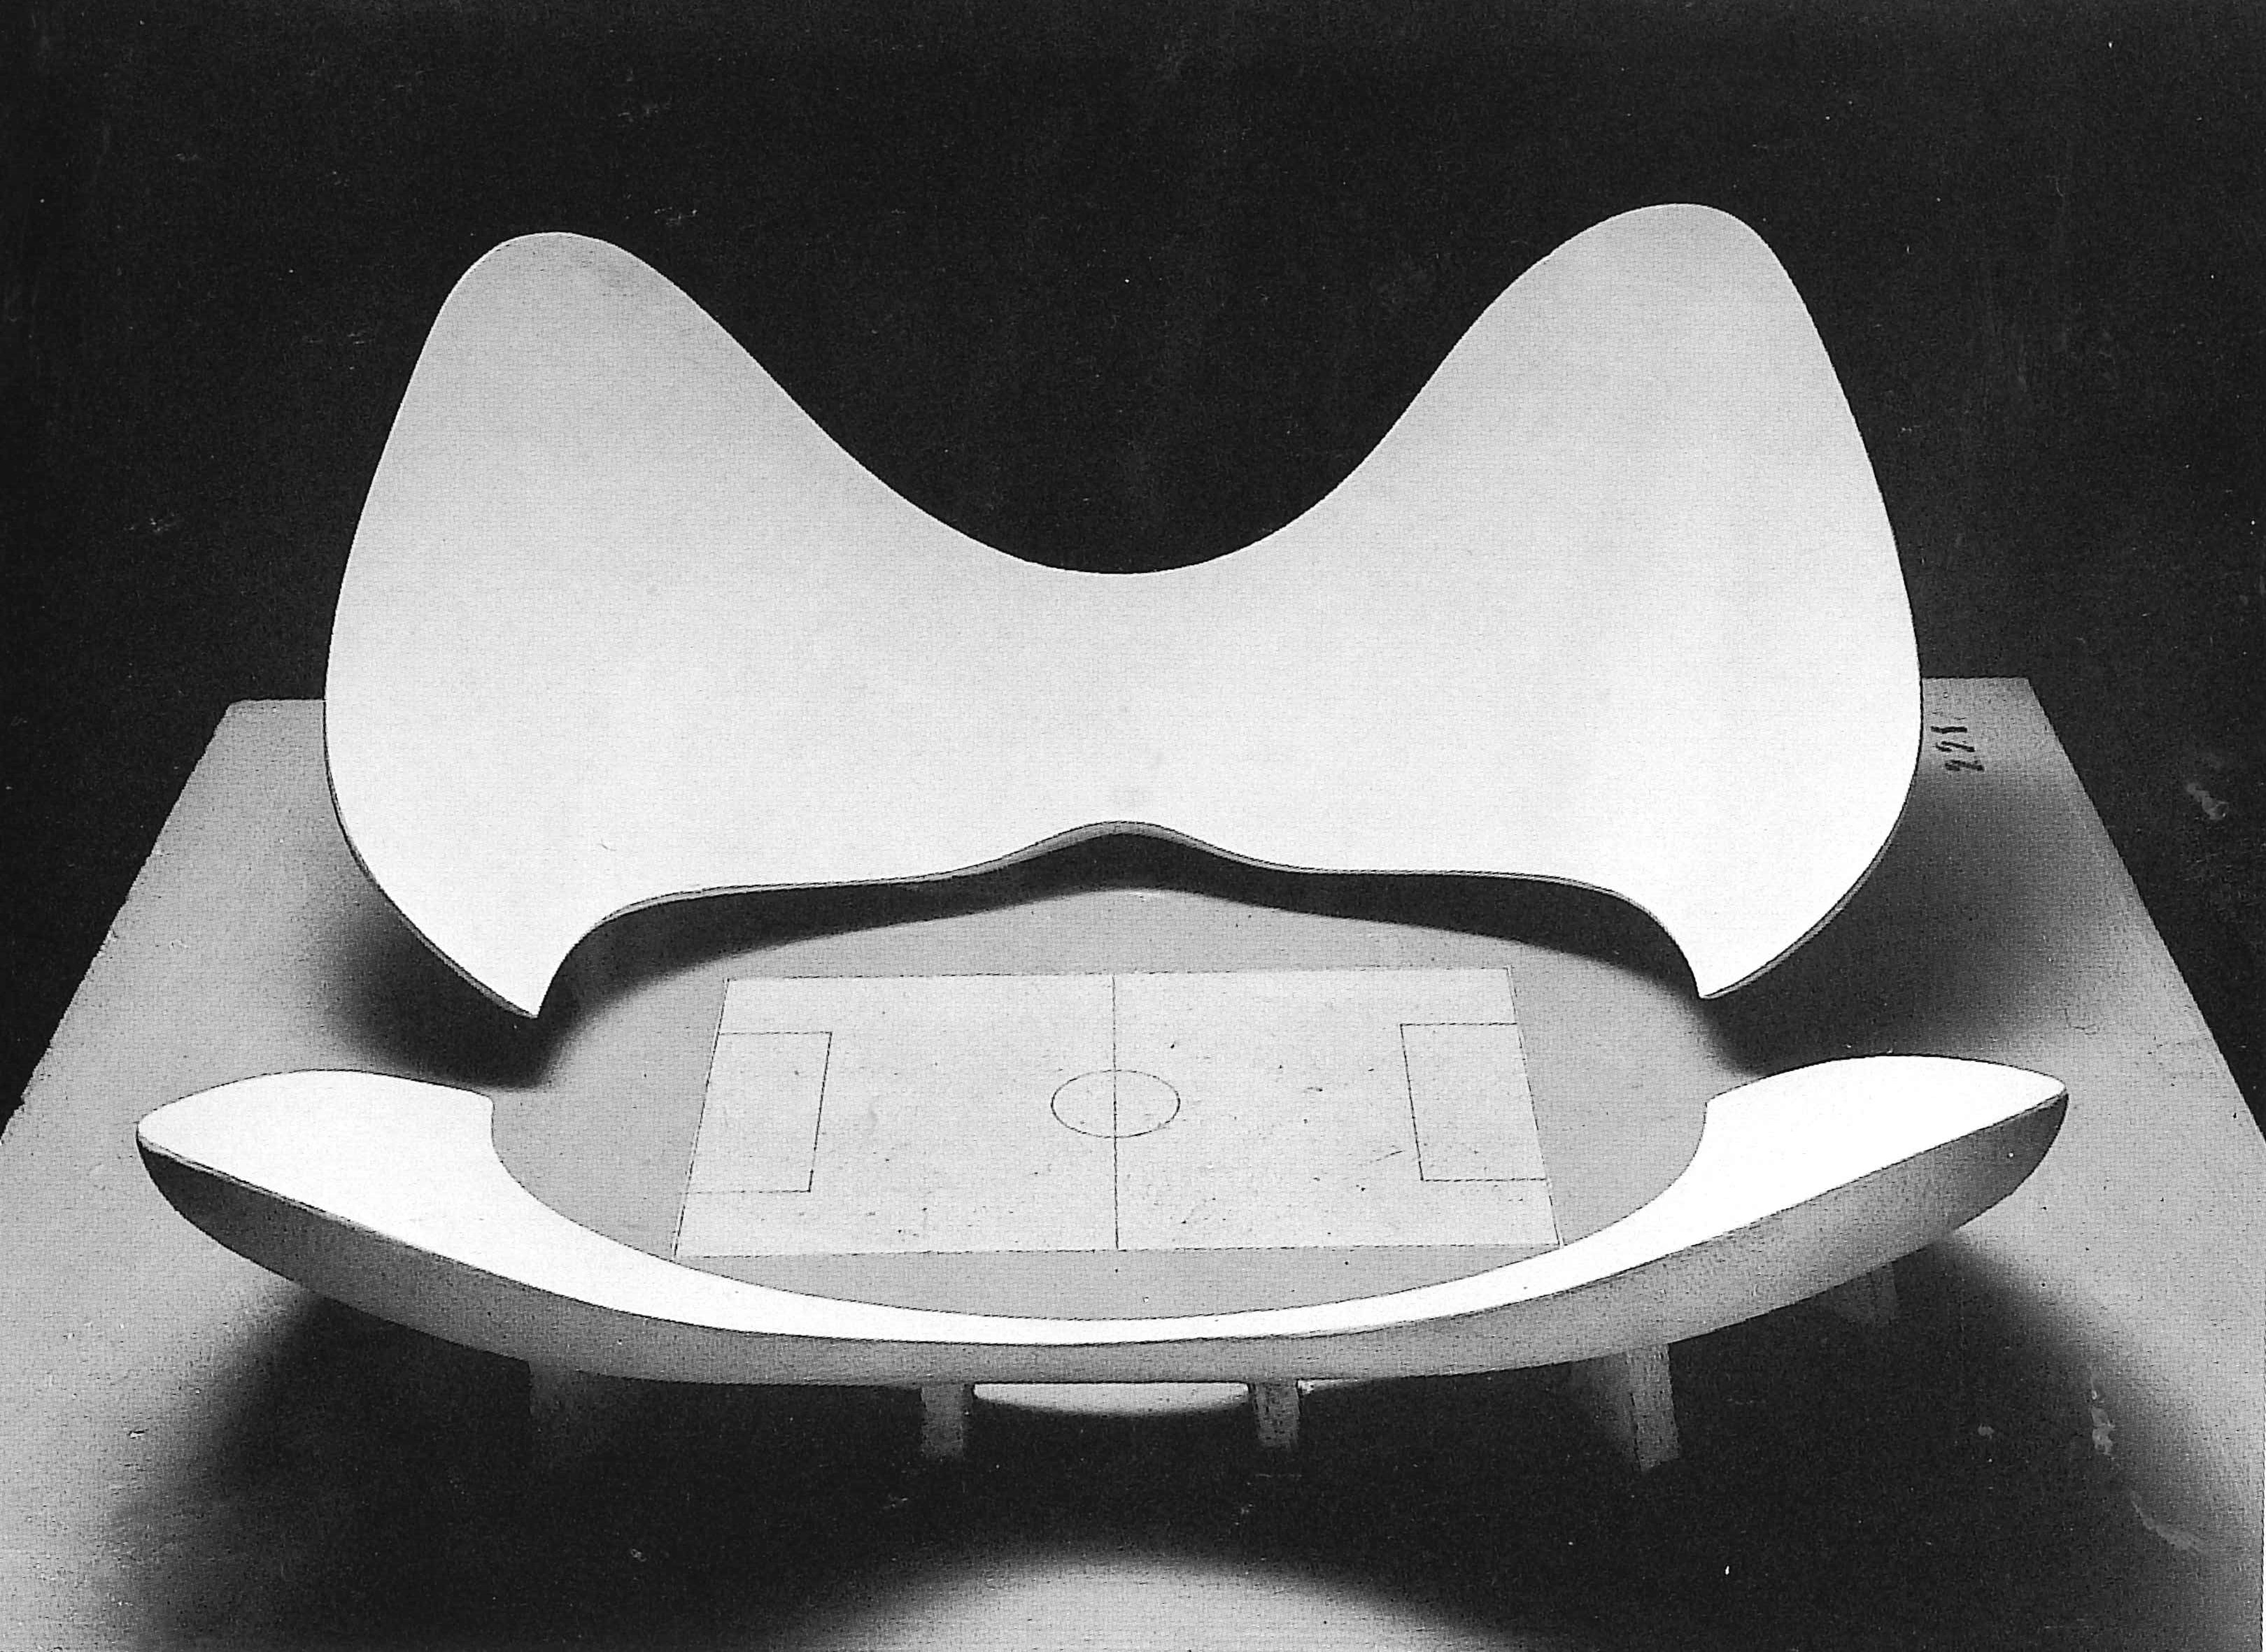
\includegraphics[width = \linewidth]{obrazky-figures/moretti_1.jpg}
    \caption{Model štadióna N od Luigi Moretti. Tento model bol vystavený na výstave parametrickej architektúry v~Twelfth Milan Triennial v~roku 1960. Parametrický model pozostávajúci z~devätnástich parametrov. Zdroj:  \cite{davis_2013}}
    \label{fig:morretiStadion}
\end{figure}

\begin{figure}[H]
    \centering
    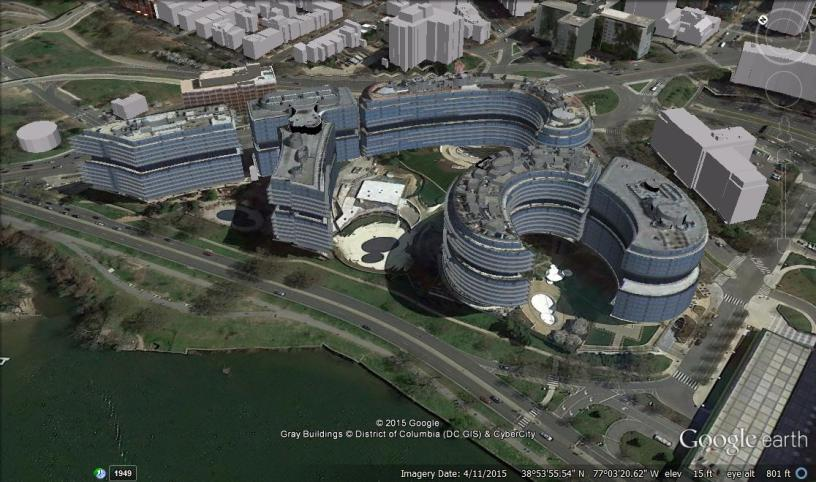
\includegraphics[width = \linewidth]{obrazky-figures/watergate-complex.jpg}
    \caption{Watergate Complex navrhnutý Luigi Morettim. Prvý veľký stavebný projekt, na ktorý boli využité parametrické modely. Zdroj: \cite{munger_2015}}
    \label{fig:Watergate}
\end{figure}





\section{Systémy pre tvorbu parametrických modelov}
Existuje niekoľko systémov pre tvorbu parametrických modelov. Zväčša sú platené, ale sú aj také, ktoré umožňujú vytváranie modelov zdarma. Väčšinou tieto parametrické modelovacie systémy nie sú navrhnuté pre domáceho používateľa ale skôr pre profesionálnych 3d dizajnérov. Táto časť je podľa blogu \cite{gaget_2018}.


\subsection*{Solidworks}
Solidworks je jedným z~najlepších softvérov na tvorbu mechanických častí. Tento parametrický softvér je profesionálny nástroj pre inžinierov a dizajnérov. Umožňuje vykonať nad vytvoreným modelom aj rôzne simulácie, napríklad záťažové alebo tepelné ako je vidieť na obrázku \ref{fig:solidworks_simulations}.



\begin{figure}[H]
    \centering
    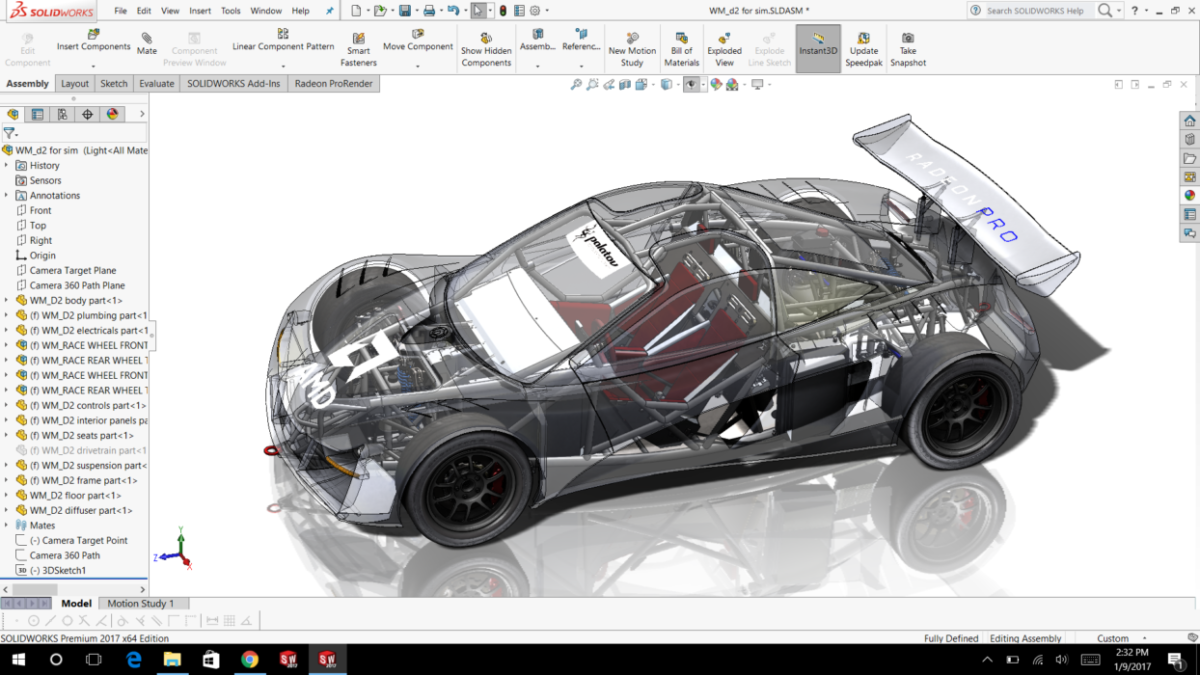
\includegraphics[width = 0.49\linewidth]{obrazky-figures/programs/solidworks_01.png}
    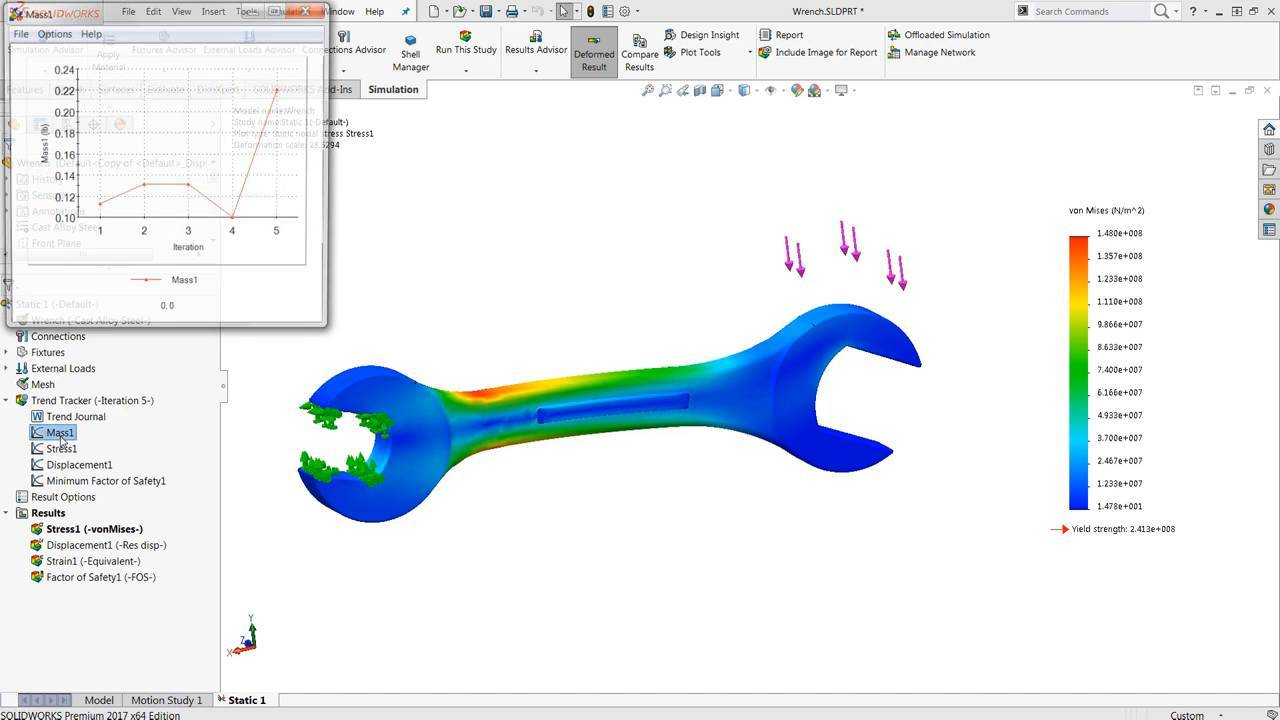
\includegraphics[width = 0.49\linewidth]{obrazky-figures/programs/solidworks, simulation.jpg}
    \caption{Prostredie programu Solidworks. Vpravo je záťažová simulácia. Zdroj: \cite{solidworks_2017} \cite{ames_2017} }
    % je tepelná simulácia \cite{goengineer_2014}
    \label{fig:solidworks_simulations}
\end{figure}


\subsection*{Catia}
Tento softvér je náročnejší pre menej zdatných užívateľov. Je to komplexný nástroj určený hlavne pre profesionálov a umožňuje množstvo pokročilejších nástrojov, ako je prevedenie 2D obrázku do 3D modelu alebo generovanie organických tvarov, ktoré spĺňajú pevnostné požiadavky, ale sú od pôvodného modelu značne odľahčené \cite{technodat_cz_2017}.

\begin{figure}[H]
    \centering
    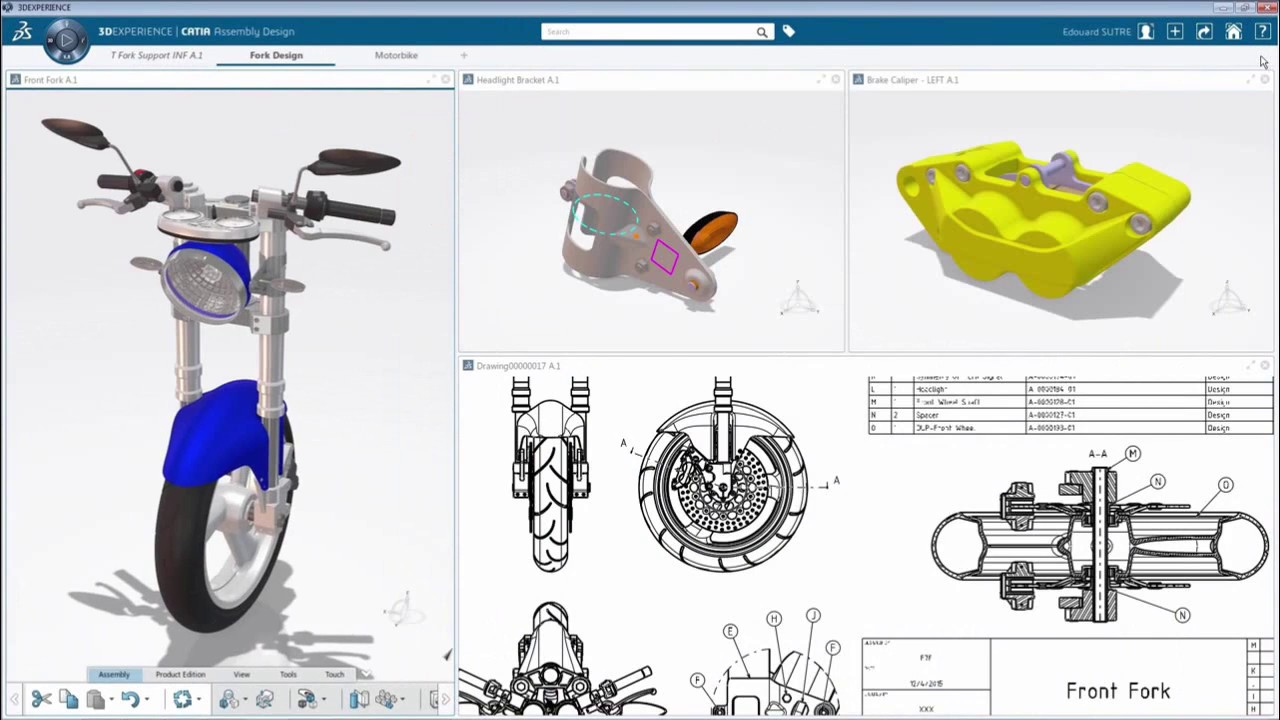
\includegraphics[width = 0.49\linewidth]{obrazky-figures/programs/Catia.jpg}
    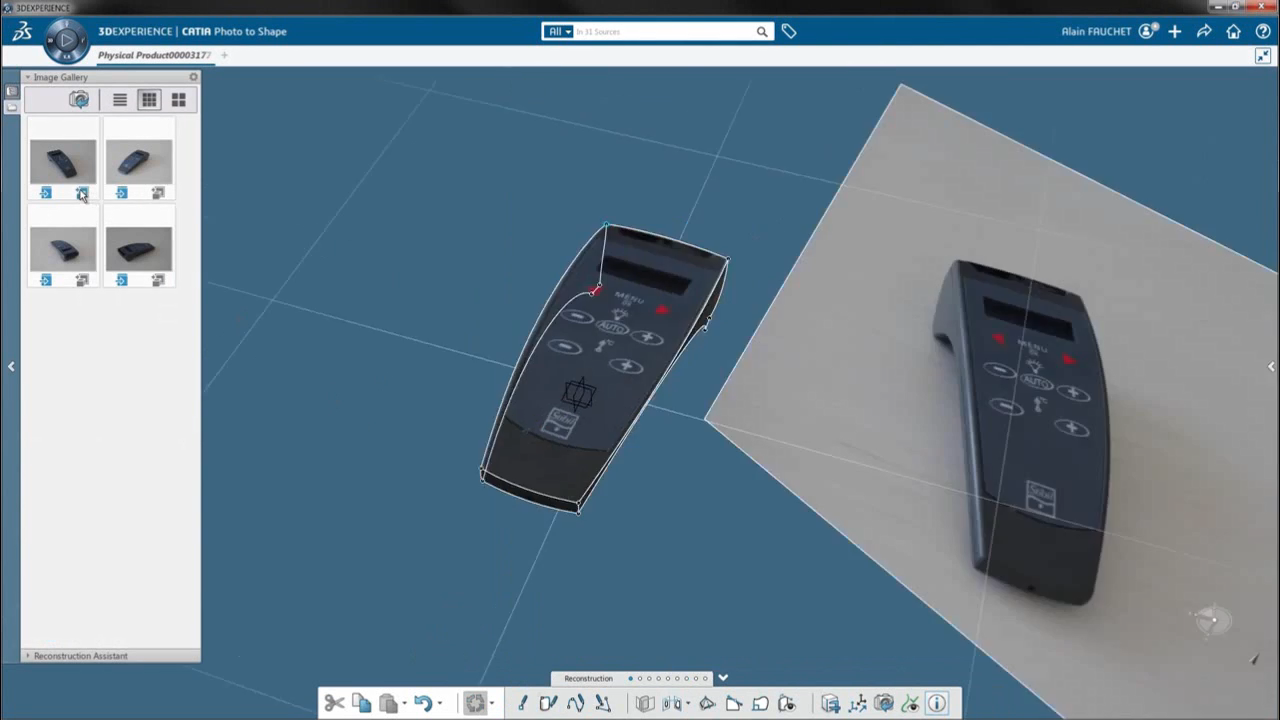
\includegraphics[width = 0.49\linewidth]{obrazky-figures/programs/Catia2.png}
    \caption{Prostredie programu Catia. Vpravo je ukážka prevodu z~2D obrázku do 3D modelu. Zdroj: \cite{technodat_cz_2017} }
    \label{fig:Catia}
\end{figure}


\subsection*{FreeCAD}
FreeCad je voľne dostupný softvér s~intuitívnym grafickým rozhraním. Umožňuje množstvo podobných nástrojov ako Catia a SolidWorks. Je zameraný na strojárstvo a návrh výrobku~\cite{freecad_2018}.

\begin{figure}[H]
    \centering
    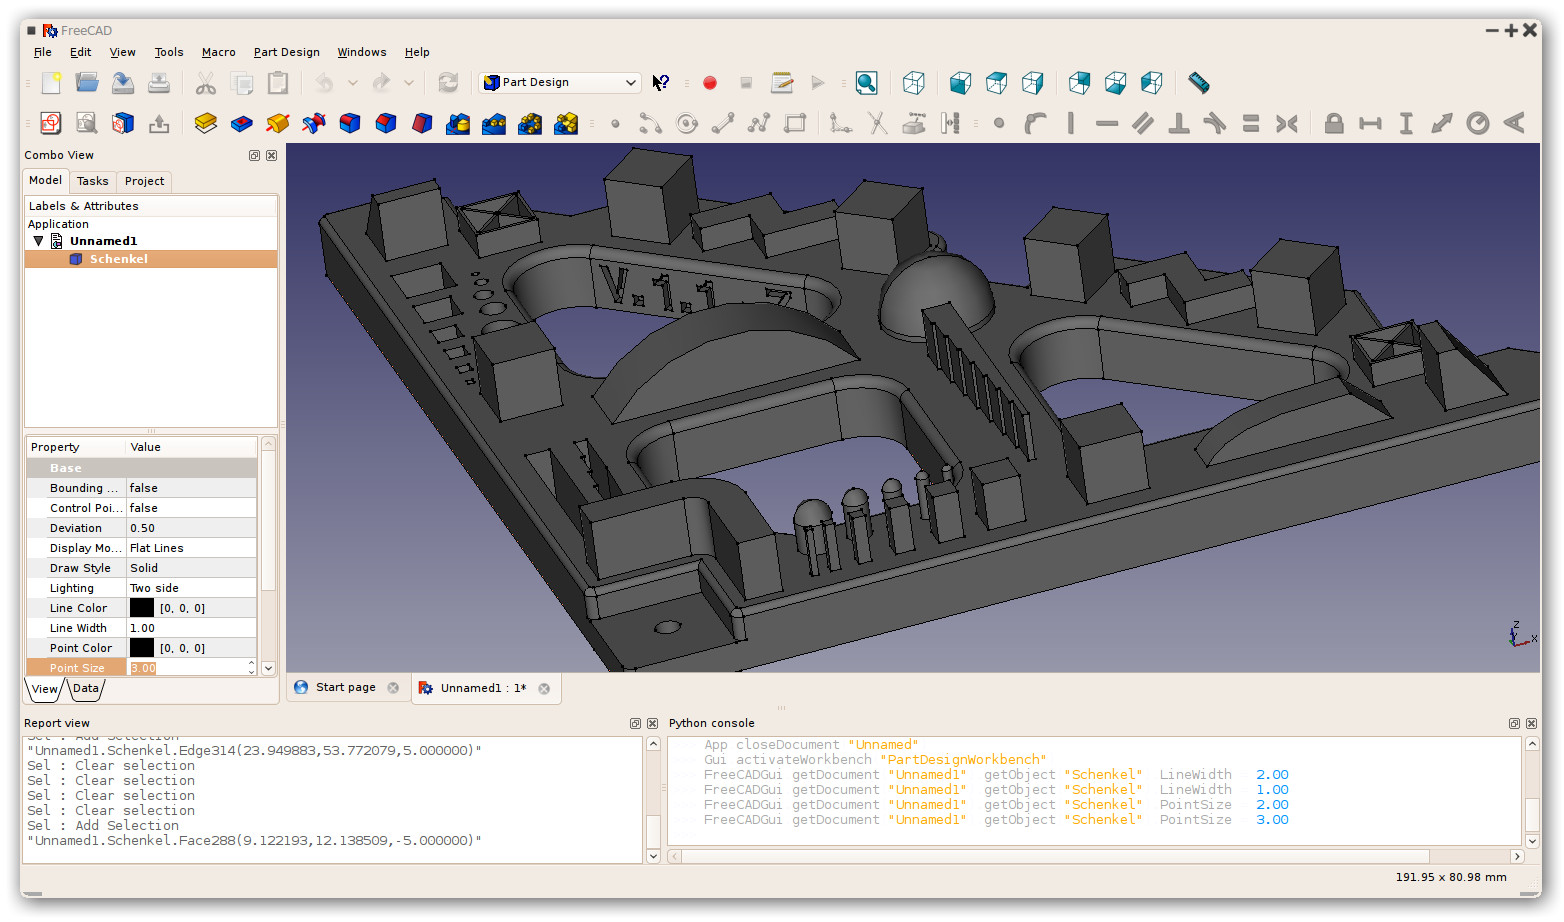
\includegraphics[width = 0.5\linewidth]{obrazky-figures/programs/Freecad_default.jpg}
    \caption{Prostredie programu FreeCAD. Zdroj: \cite{freecad_2018}}
    \label{fig:FreeCAD}
\end{figure}


\subsection*{Creo Parametric}
Jedná sa o~softvér pre priemyselný dizajn. Umožňuje vytvárať zložité 3d modely. Poskytuje veľa účinných nástrojov prispôsobených priemyselnému výrobnému prostrediu. Tento softvér sa často používa napríklad v~automobilovom priemysle.

\begin{figure}[H]
    \centering
    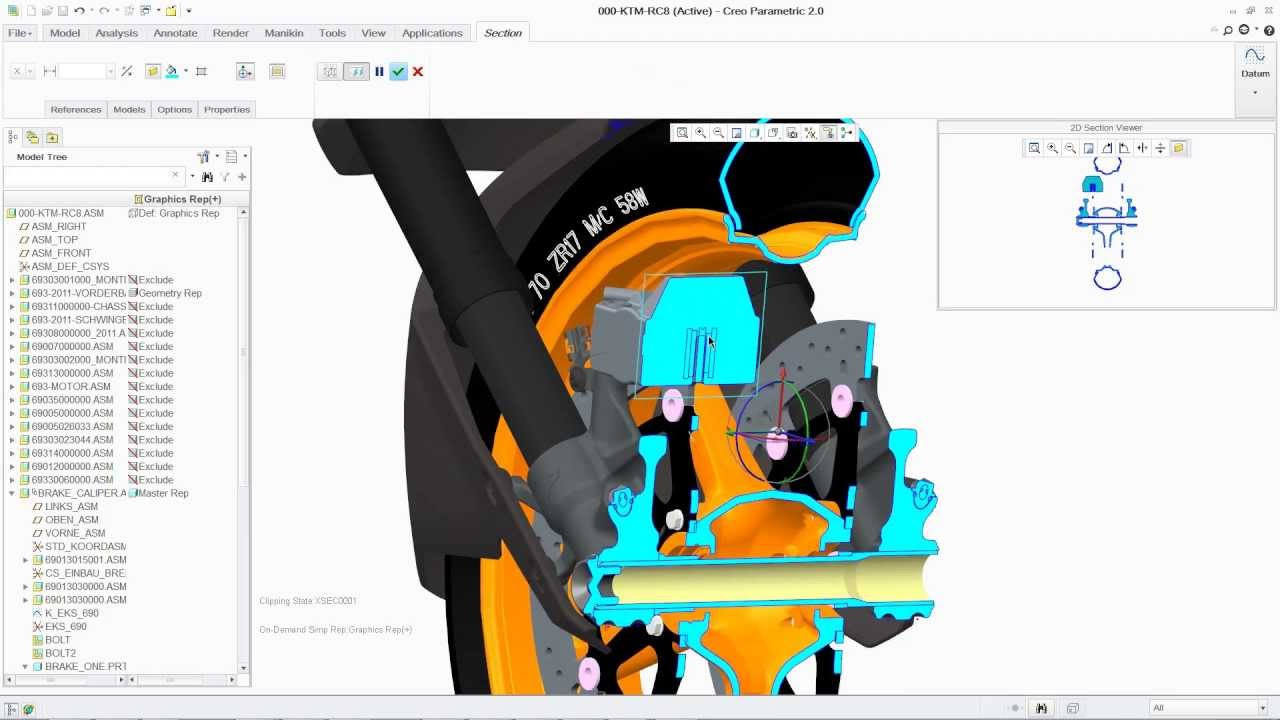
\includegraphics[width = 0.5\linewidth]{obrazky-figures/programs/Creo_Parametric.jpg}
    \caption{Prostredie programu Creo Parametric Zdroj: \cite{ptc_2013} }
    \label{fig:Creo}
\end{figure}


\subsection*{Rhino s~plugiom Grasshopper}
Rhino je profesionálny 3D CAD softvér používaný v~množstve spoločností. Pre prácu s~parametrickými modelmi je potrebný plugin Grasshopper. 

Grasshopper je vizuálny programovací jazyk, znázornený na obrázku \ref{fig:Grasshopper}.
Umožňuje tvorbu parametrických modelov pre konštrukčné inžinierstvo, architektúru a výrobu.

\begin{figure}[H]
    \centering
    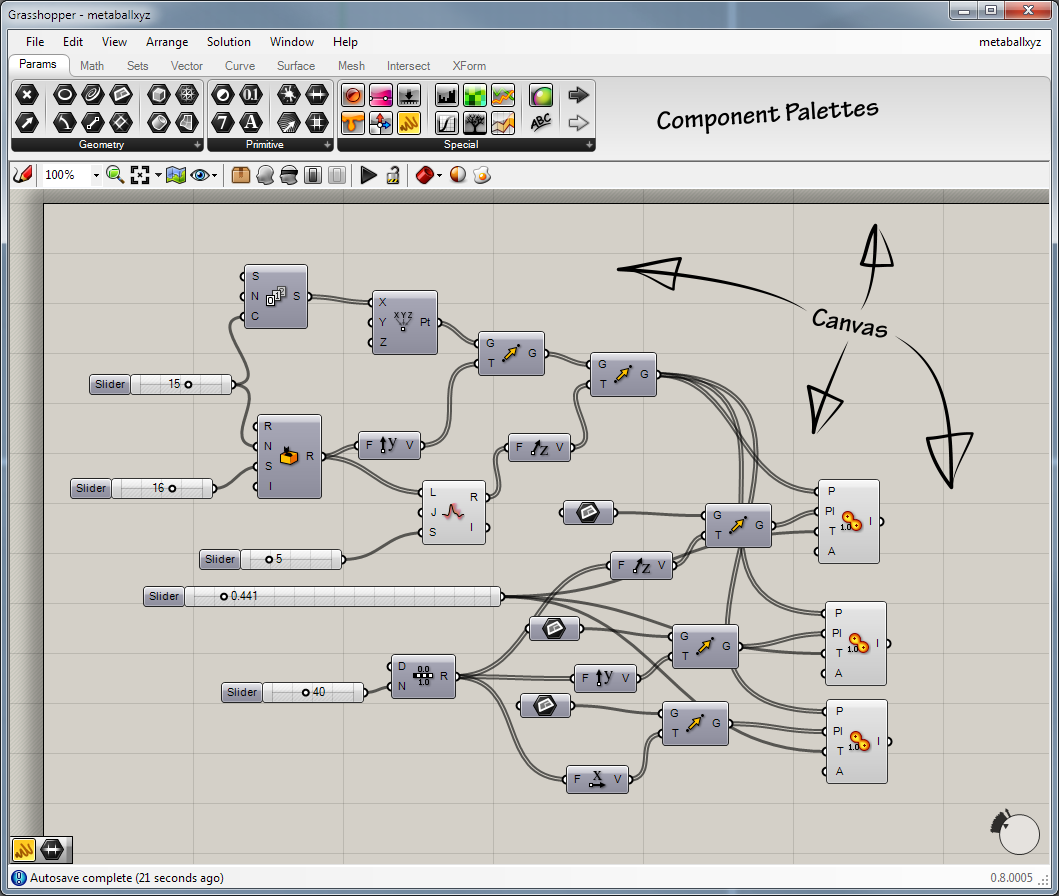
\includegraphics[width = 0.5\linewidth]{obrazky-figures/programs/Grasshopper_MainWindow.png}
    \caption{Prostredie programu Grasshopper Zdroj: \cite{rutten_2011} }
    \label{fig:Grasshopper}
\end{figure}


\subsection*{Fusion 360}
Fusion 360 nie je iba  parametrický modelovací systém. Podporuje aj priame modelovanie a umožňuje prechod medzi týmito typmi modelovania. Keďže pri priamom modelovaní nie je model vytváraný pomocou stromu operácií, je tento strom pri prenose odstránený. Má dobré simulačné a modelovacie nástroje, ktoré pomáhajú pri návrhu.

\begin{figure}[H]
    \centering
    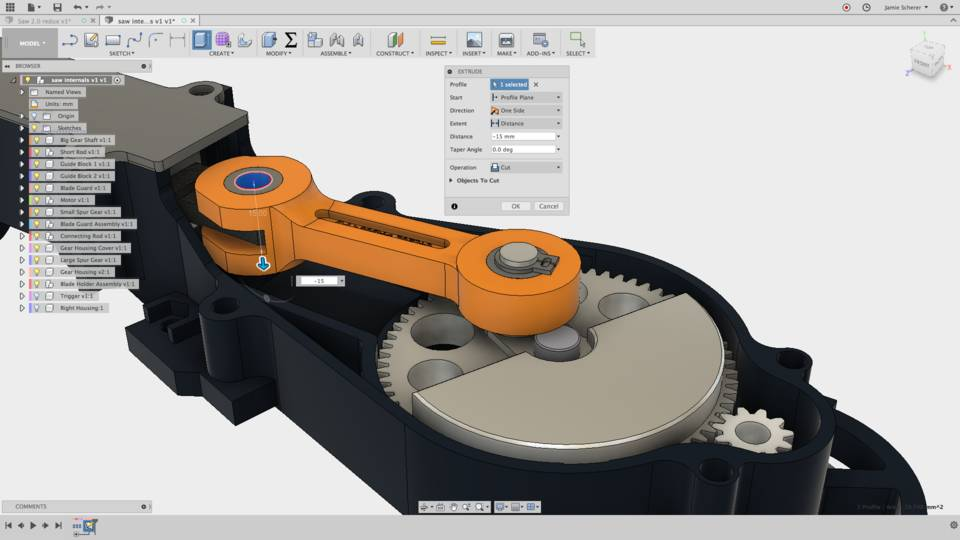
\includegraphics[width = 0.5\linewidth]{obrazky-figures/programs/Fusion.jpg}
    \caption{Fusion 360 Zdroj: \cite{gaget_2018} }
    \label{fig:Fusion}
\end{figure}

\subsection*{Inventor}

Inventor je rovnako ako Fusion 360 vytvorený spoločnosťou Autodesk. Tento program je často používaný v~strojárstve. Inventor ponúka množstvo parametrických možností, ktoré pomáhajú vytvárať 3D modely a hlavne mechanické konštrukcie.


\begin{figure}[H]
    \centering
    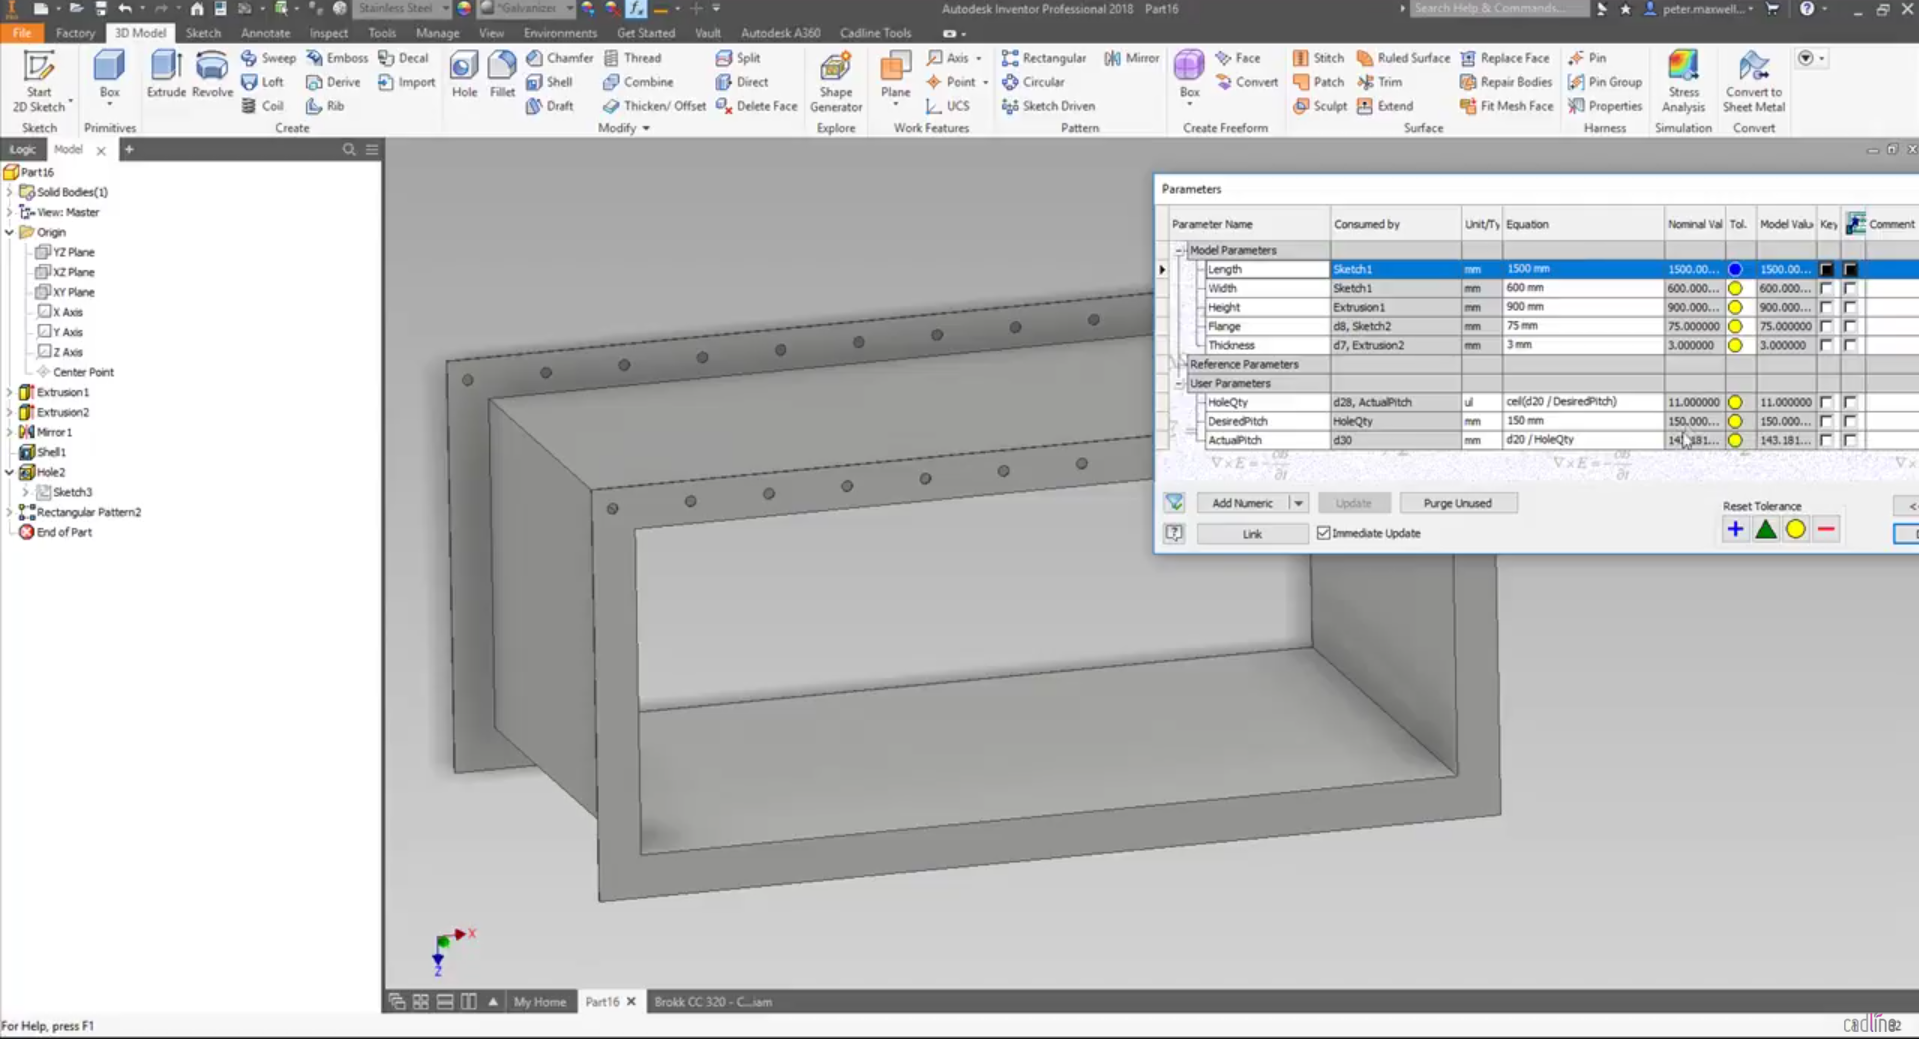
\includegraphics[width = 0.5\linewidth]{obrazky-figures/programs/Inventor.png}
    \caption{Fusion 360 Zdroj: \cite{cadline_2017} }
    \label{fig:Inventor}
\end{figure}


\chapter{Geometrické objekty a operácie}
\label{chapt:Geometrické_tvary}

Geometrické objekty môžeme rozdeliť do 4 kategórií podľa dimenzií. Body, úsečky, plochy a objemové objekty.
Zložitejšie objekty z~vyšších rozmerov sú tvorené z~objektov z~nižších rozmerov. 
%Parametre objektov  podľa toho do akej kategórie patria. 
Niektoré geometrické objekty majú podobné parametre. Všetky plošné útvary majú normálu, stred a aj plochu a obvod. Každý geometrický objekt má svoje meno a priehľadnosť. Tieto parametre pre geometrické objekty sa dajú zobraziť pomocou stromu dedičnosti. Ten je zobrazený na obrázku \ref{fig:StromDedicnosti}. 
Jednotlivé geometrické objekty obsahujú hodnoty, ktoré sa zadávajú a hodnoty, ktoré sa dajú vypočítať. Napríklad ihlan s~kruhovou podstavou obsahuje stred a polomer základne a výšku ihlanu. Vypočítanými hodnotami sú obvod a obsah základne alebo objem a plocha ihlanu.  

Táto kapitola pokračuje opisom jednotlivých geometrických objektov a operácií, ktoré ich vytvárajú.

\begin{figure}[]
	\centering
	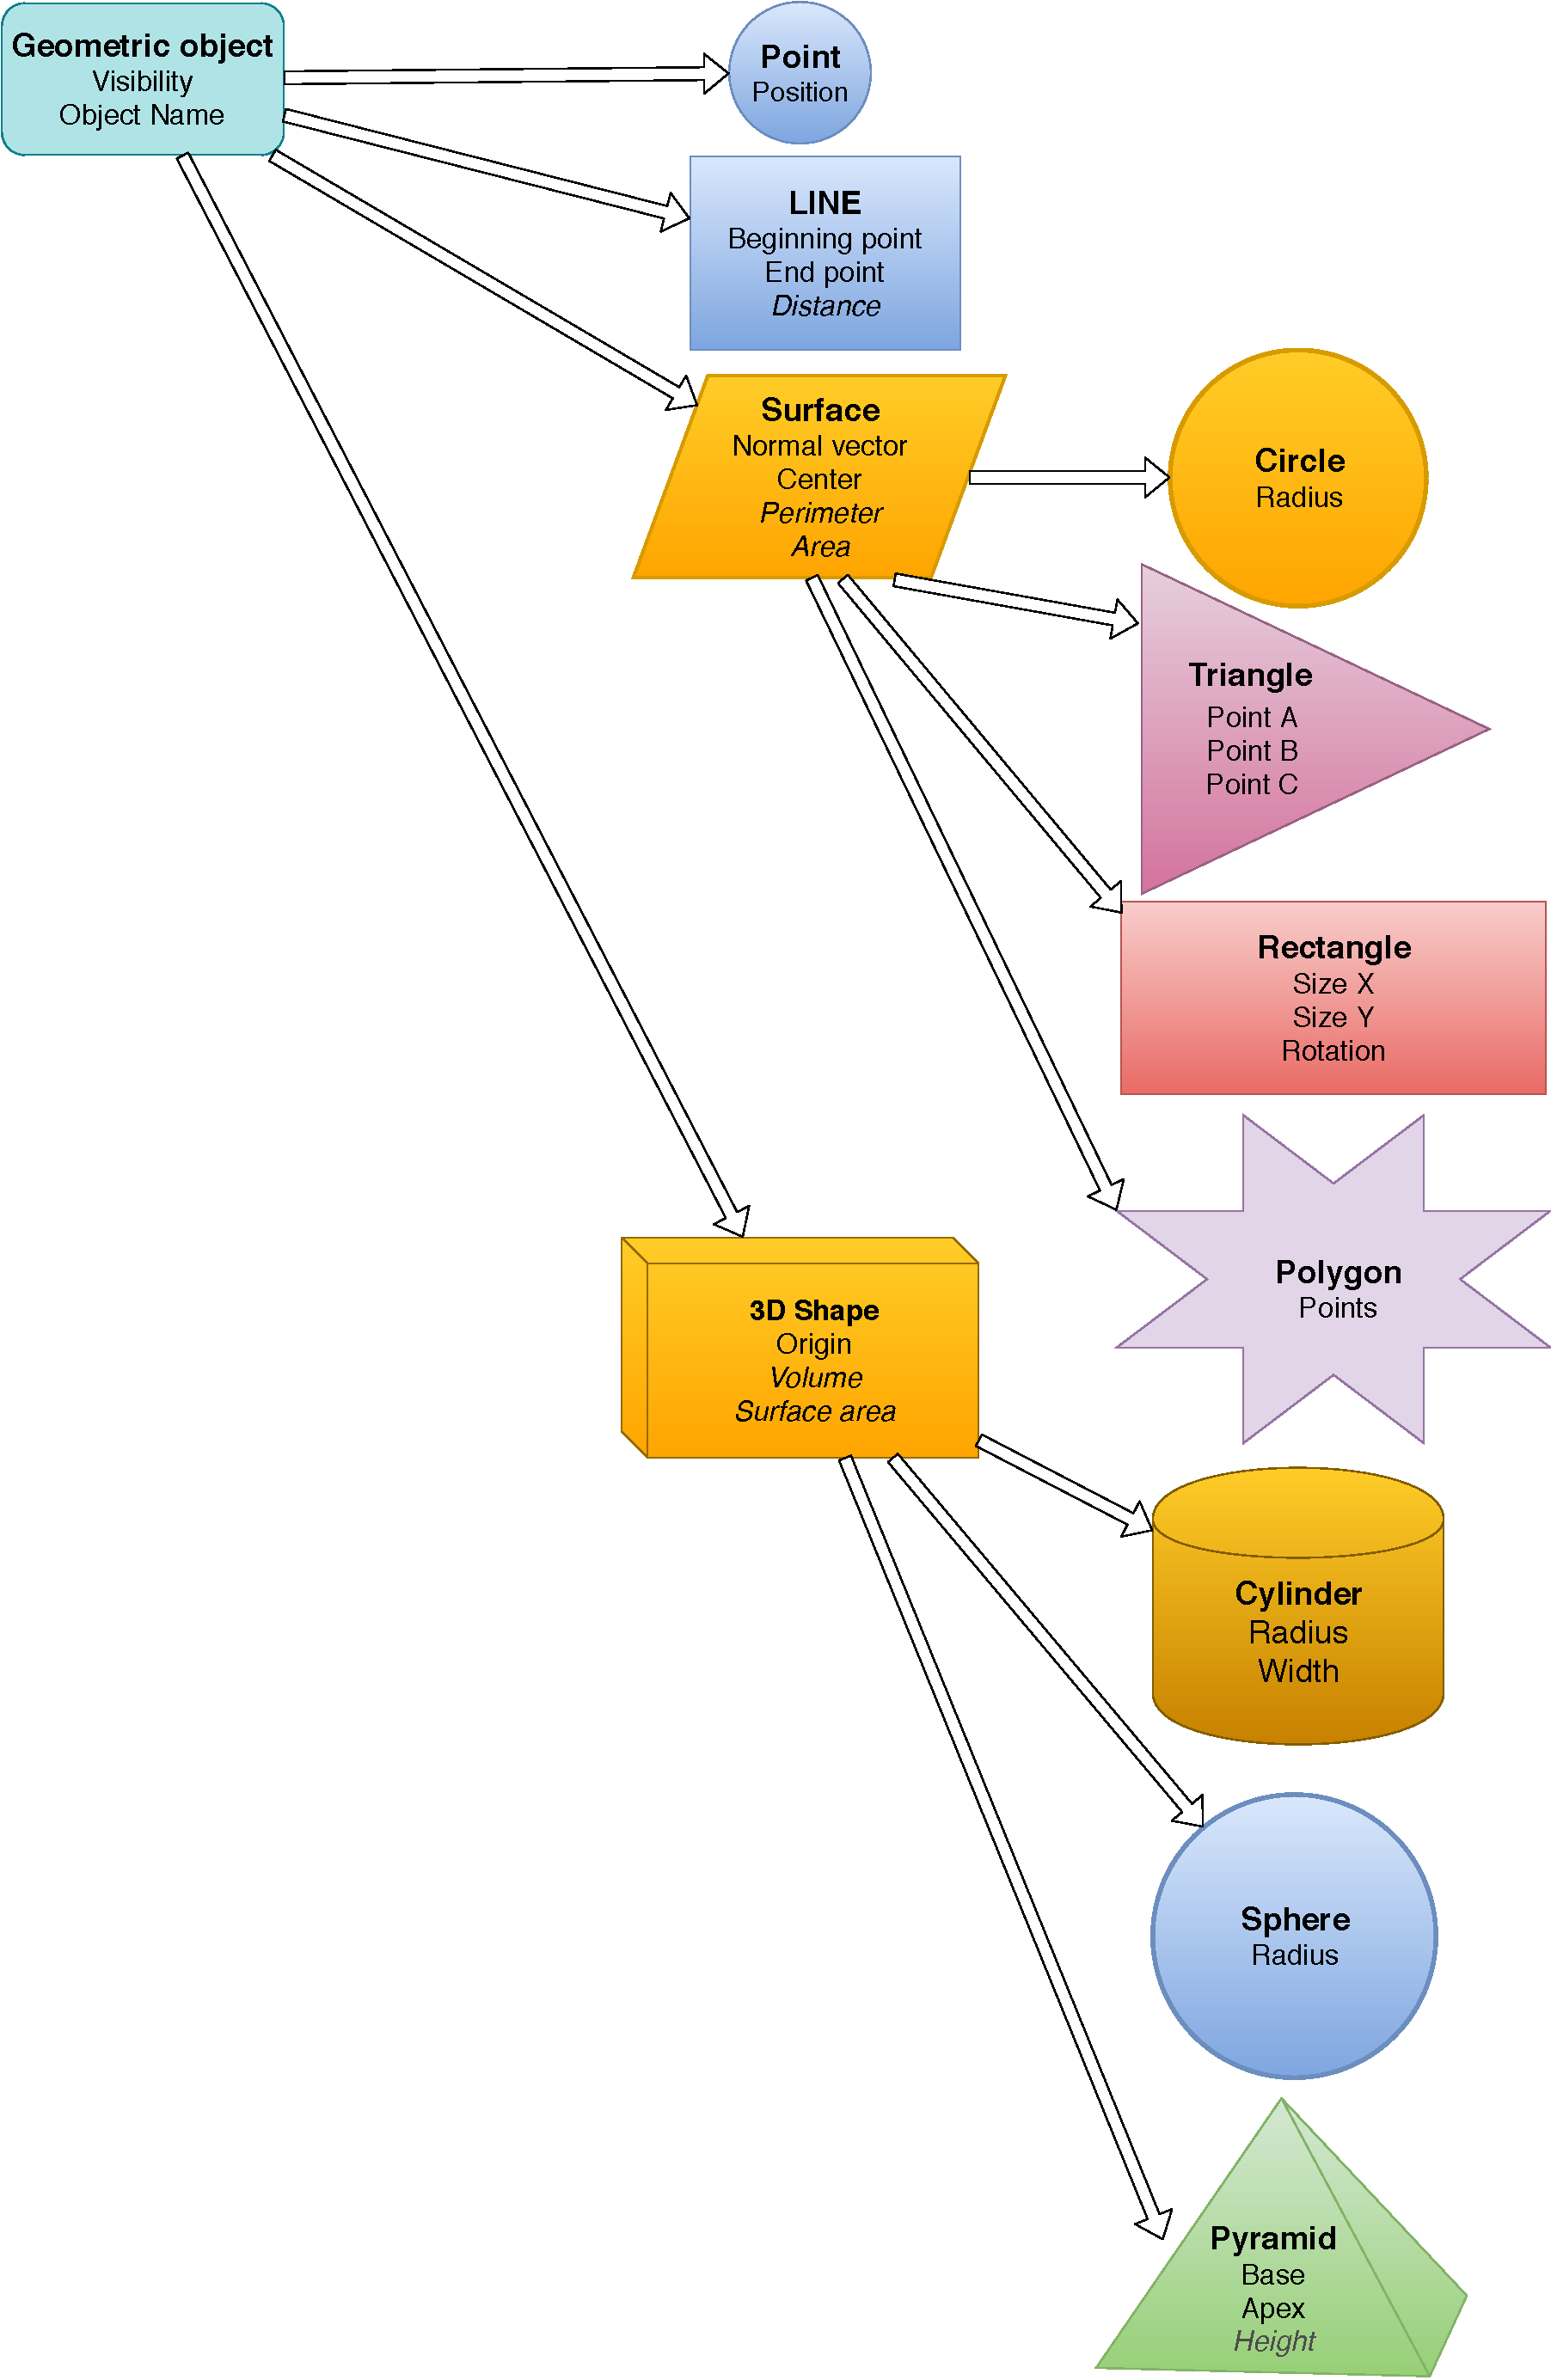
\includegraphics[height=0.95\textheight]{obrazky-figures/Diagram/Draw/DP Navrh operacii-Structure.pdf}
	\caption{Štruktúry objektov vytvárajú strom dedičnosti. Pri každom objekte je uvedené, aké dáta uchováva. }
	\label{fig:StromDedicnosti}
\end{figure}

\section{Bod}
Bod je základnou stavebnou jednotkou všetkých objektov. Všetky geometrické útvary sa dajú definovať ako množina bodov. Je to bezrozmerný geometrický útvar, teda nemá šírku, výšku ani hrúbku. Jeho úlohou je označiť pozíciu v~priestore. Pozíciu bodu v~trojrozmernom priestore udáva vzdialenosť na jednotlivých osiach ortogonálneho súradnicového systému X, Y a Z. Táto pozícia môže byť v~absolútnom tvare, teda od stredu súradnicového systému alebo v~relatívnom tvare, kedy je závislá na pozícii iného bodu.



\begin{figure}[H]
	\centering
	%\subfloat{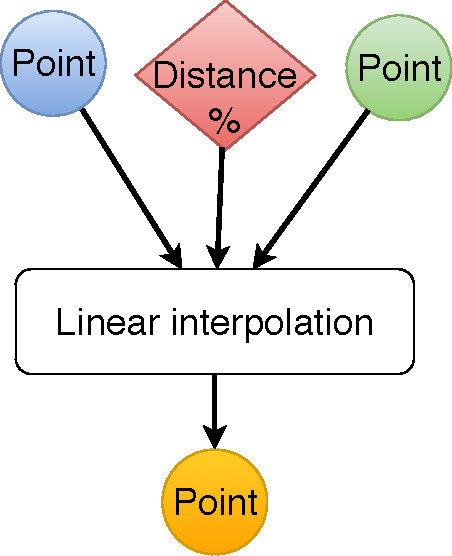
\includegraphics[height=0.3\textwidth]{obrazky-figures/Diagram/Point/DP Navrh operacii-0D - Point Linear interpolation.pdf}}
	\subfloat{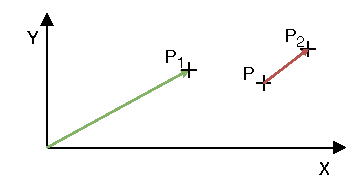
\includegraphics[height=0.3\textwidth]{obrazky-figures/Diagram/Draw/1Points/DP Navrh operacii-0D - Point.pdf}}
	\caption{Bod P$_1$ s~absolútnou pozíciou a bod P$_2$ s~relatívnou pozíciou od bodu P}
	\label{fig:Point}
\end{figure}
\subsection*{Lineárna interpolácia}
Lineárna interpolácia umožňuje získať bod, ktorý je na rovnakej priamke ako dva zadané body. Na obrázku \ref{fig:PointLinearInterpolation} sú tieto body zobrazené modrou a zelenou farbou, výsledný bod je zobrazený žltou farbou. Pozícia bodu závisí od zadanej vzdia\-le\-nos\-ti od počiatočného bodu. Táto vzdia\-le\-nosť môže byť zadaná dĺžkou alebo percentuálne, kde 50\% vytvorí bod uprostred počiatočného a koncového bodu. 




\begin{figure}[H]
	\centering
	%\subfloat{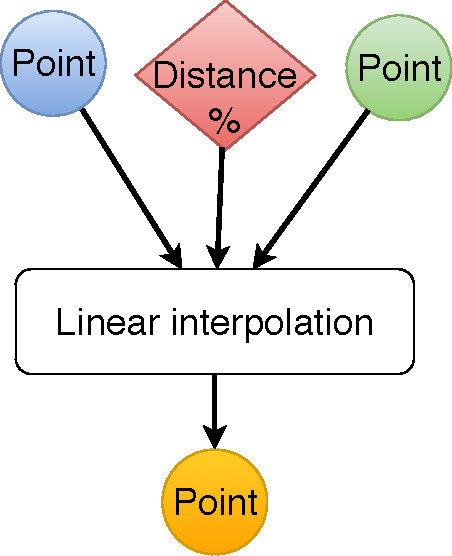
\includegraphics[height=0.3\textwidth]{obrazky-figures/Diagram/Point/DP Navrh operacii-0D - Point Linear interpolation.pdf}}
	\subfloat{
\includegraphics[height=0.3\textwidth]{obrazky-figures/Diagram/Draw/1Points/DP Navrh operacii-0D - PointLinearInterpolation.pdf}}
	\caption{Lineárna interpolácia medzi bodmi.  \texttt{d} označuje vzdialenosť medzi zadanými bodmi a  \texttt{h} označuje vzdialenosť v~akej sa má vykonať interpolácia }
	\label{fig:PointLinearInterpolation}
\end{figure}

Ak je zadaná vzdialenosť pomocou dĺžky, použije sa vzorec \ref{eq:LiearnInterpolation}. Pri percentuálnej vzdialenosti sa použije obdobný vzorec, ale vektor medzi bodmi bod1 a bod2 sa nenormalizuje.
\begin{equation}
    bod = bod1 + norm(bod2 - bod1) * vzdialenos\check{t};
	\label{eq:LiearnInterpolation}
\end{equation}


\subsection*{Priesečník plochy a úsečky}

Pri tejto operácii sa používa ľubovolný plošný objekt ako rovina a úsečka ako priamka. Táto geometrická operácia vytvorí bod v~mieste, kde sa priamka pretína s~rovinou. 


\begin{figure}[H]
	\centering
	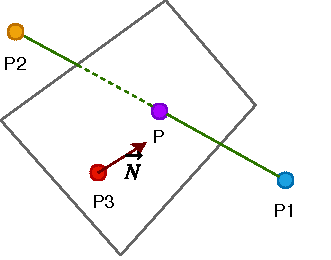
\includegraphics[height=0.3\textwidth]{obrazky-figures/DP Navrh operacii-Intersection.pdf}
	\caption{Pretnutie plochy priamkou}
	\label{fig:Intersection}
\end{figure}


Rovnica pre rovinu, ktorá je tvorená bodom \texttt{P\textsubscript{3}} nachádzajúcom sa na rovine a normálou N, sa dá zapísať ako \ref{eq:rovnicaPlochy_intersection} \cite{bourke_Point_Line_Plane}. 
\begin{equation}
    \textbf{N} \cdot (\textbf{P} - \textbf{P3}) = 0
	\label{eq:rovnicaPlochy_intersection}
\end{equation}
Rovnica priamky \ref{eq:rovnicaPriamky_intersection}, ktorá je určená bodmi \texttt{P\textsubscript{1}} a \texttt{P\textsubscript{2}}
\begin{equation}
	\textup{P}=\textbf{P1}+u (\textbf{P2}-\textbf{P1})
    \label{eq:rovnicaPriamky_intersection}
\end{equation}
Bod \texttt{P} označuje priesečník medzi rovinou a priamkou. Pomocou substitúcie získame rovnicu \ref{eq:rovnicaPriesecniku}.
\begin{equation}
	\textbf{N} \cdot (\textbf{P1}+u(\textbf{P2}-\textbf{P1}))) = \textbf{N} \cdot \textbf{P3}
    \label{eq:rovnicaPriesecniku}
\end{equation}
Po vyriešení tejto rovnice dostaneme rovnicu \ref{eq:rovnicaPriesecnikuSolved}. Výslednú pozíciu bodu dostaneme dosadením $u$ do rovnice pre  priamku \ref{eq:rovnicaPriamky_intersection}.
\begin{equation}
	u=\frac
{\textbf{N} \cdot (\textbf{P3}-\textbf{P1})}
{\textbf{N} \cdot (\textbf{P2}-\textbf{P1})}
    \label{eq:rovnicaPriesecnikuSolved}
\end{equation}


Ako je vidieť na obrázku \ref{fig:GraphIntersection_Plane_Line}, pomocou tejto operácie sa vytvorí bod aj mimo zadaných objektov. Problém nastáva, ak je zadaná úsečka paralelná s~plochou a teda je kolmá na normálu plochy $N$. Skalárny súčin v~menovateli je potom rovný 0. V~tomto prípade priesečník buď neexistuje, alebo je priesečníkov nekonečne veľa, ak úsečka leží na rovine.

\begin{figure}[H]
	\centering
%	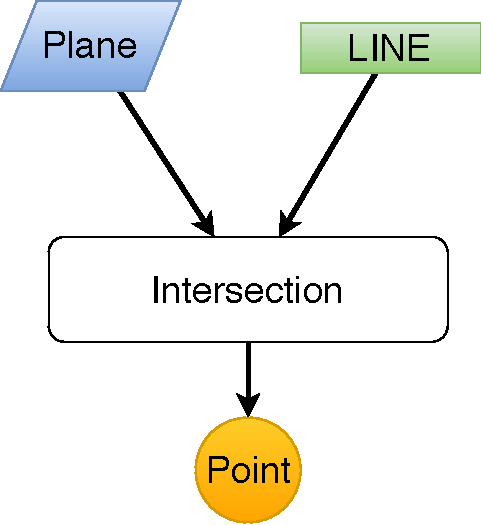
\includegraphics[height=0.3\textwidth]{obrazky-figures/Diagram/Point/DP Navrh operacii-0D - PointIntersection PlaneLine.pdf}
	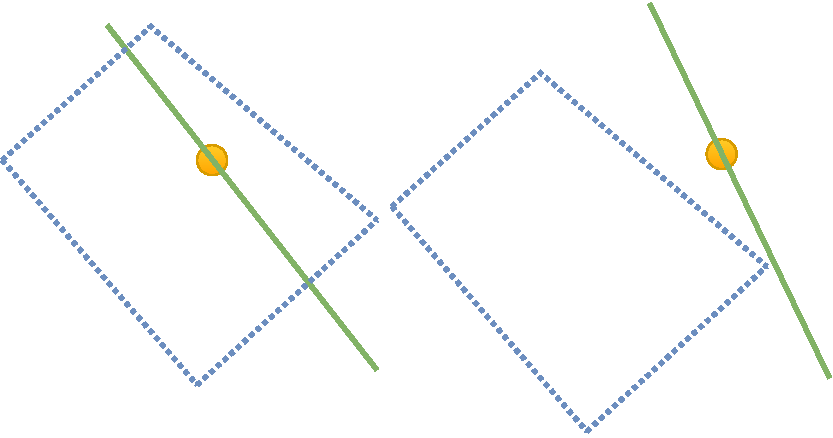
\includegraphics[height=0.3\textwidth]{obrazky-figures/Diagram/Draw/1Points/DP Navrh operacii-0D - PointIntersectionPlaneLine.pdf}
	\caption{Priesečník plochy a priamky. Vpravo je zobrazený prípad, ak sa priesečník nachádza na rovine, ale mimo plochy objektu}
	\label{fig:GraphIntersection_Plane_Line}
\end{figure}

\subsection*{Stred plochy}
Existuje množstvo možností ako získať stred objektu. Do tejto práce som vybral dve metódy a to metódu minimálneho štvorca a priemer všetkých bodov. %Pri týchto operáciách sa prevádza zadaná plocha z trojrozmerného priestoru  do dvojrozmerného.


\subsubsection{Minimálny štvorec}
Pri tejto operácii sa prejdú všetky body a zistí sa maximálna a minimálna hodnota v~jednotlivých osiach a výsledný bod sa nachádza uprostred nich.

%//Create point on position of middle of entered surface
%	//	Example:
%	//		SurfaceMiddle(PointName, Circle)	//- Create Point on center of Circle
%	//		SurfaceMiddle(PointName, Rectangle)	//- Create Point on middle of Rectangle
%	//		SurfaceCenter(PointName, Shape)		//- Create Point on middle of shape 
%	//		SurfaceMiddle(PointName, Shape)		//- Create Point on middle of shape - centroid (sum of points / count of points)

\begin{figure}[H]
	\centering
%	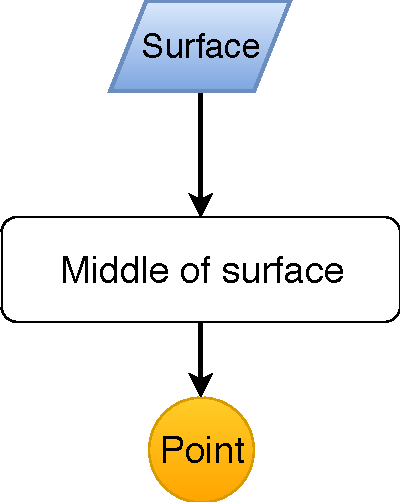
\includegraphics[height=0.3\textwidth]{obrazky-figures/Diagram/Point/DP Navrh operacii-0D - PointMiddle of surface.pdf}
	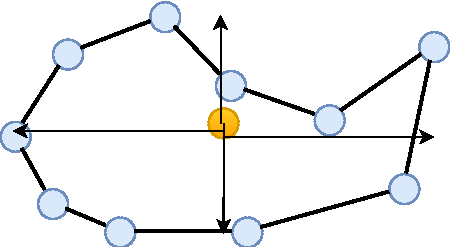
\includegraphics[height=0.3\textwidth]{obrazky-figures/Diagram/Draw/1Points/DP Navrh operacii-0D - PointMiddle of surface.pdf}
	\caption{Stred plochy pomocou minimálneho štvorca }
	\label{fig:PointMiddleofsurface}
\end{figure}



\subsubsection{Priemer všetkých bodov}
Nájdenie aritmetického priemeru všetkých bodov polygónu.

\begin{equation}
    \frac{1}{n} \sum_{i=0}^{n} p_i   
    \label{eq:aritPriemer}
\end{equation}


\subsubsection{Stred trojuholníka}
Aj pre trojuholník existuje množstvo typov stredu. V~súčastnosti je podľa encyklopédie stredov trojuholníkov známych až 30 714 trojuholníkových centier \cite{kimberling_2019}. Tento počet každým dňom narastá. Pre porovnanie, v~roku 1994 bolo známych 101, v~roku 1998 bolo 360 a v~decembri 2004 bolo známych 3053 \cite{Kimberling_Center_2004}. Medzi najznámejšie patria ťažisko (G), ortocentrum (H), stred vpísanej kružnice (I), opísanej kružnice (O) aj stred kružnice deviatich bodov (N). Tieto body sú zaznačené na obrázku \ref{fig:TriangleCenters}.


\begin{figure}[H]
	\centering
	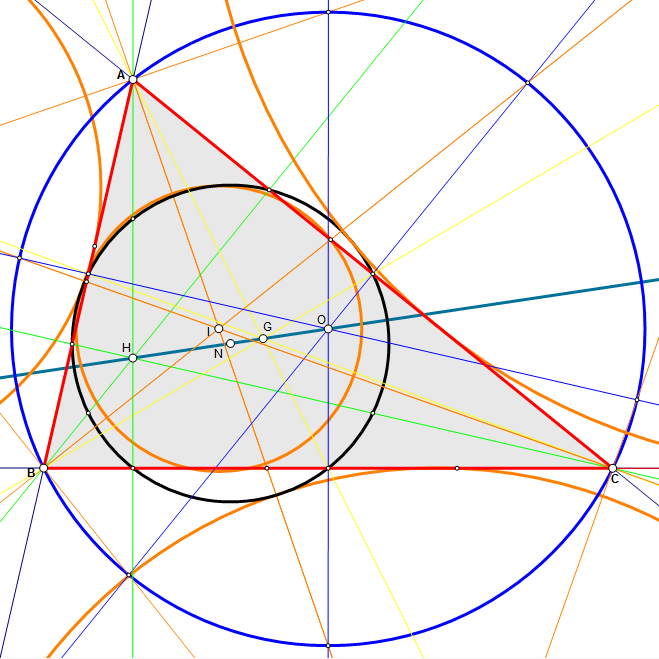
\includegraphics[width=0.9\textwidth]{obrazky-figures/Trigonometric_centres.png}
	\caption{Najznámejšie stredy trojuholníka sú ťažisko (G), ortocentrum (H), stred vpísanej kružnice (I), opísanej kružnice (O) aj stred kružnice deviatich bodov (N) \cite{triangle_center_2012}}
	\label{fig:TriangleCenters}
\end{figure}


\paragraph{Ťažisko (Centroid)}\unskip \mbox{} \\*

Ťažisko trojuholníka sa nachádza v~priesečníku troch mediánov trojuholníka. Na nájdenie jeho pozície stačí vypočítať aritmetický priemer vrcholov trojuholníka v~jednotlivých osiach \ref{eq:triangleCentroid} \cite{Centroid_of_a_Triangle}.



\begin{equation}
    \frac{A+B+C}{3}
    \label{eq:triangleCentroid}
\end{equation}

 \mbox{} \\*
\paragraph{Stred vpísanej kružnice (Incenter)}\unskip \mbox{} \\*
\label{sec:TriangleCenter}

Z~každého bodu trojuholníka urobíme priamku tak, aby uhly na oboch stranách priam\-ky boli rovnaké. Táto priamka sa nazýva tiež bisektor \cite{angle_bisector_theorem}. Stred vpísanej kružnice je na priesečníku týchto priamok.




Stred vpísanej kružnice sa dá vypočítať aj pomocou vzorca \ref{eq:Incenter}, kde  $A$, $B$, $C$ sú vrcholy trojuholníka a $a$, $b$, $c$ sú dĺžky strán protiľahlých k~vrcholom $A$, $B$, $C$. \cite{Incenter_page_2011}.
\begin{equation}
O = \frac{a\ast A+b\ast  B +c \ast C}{a + b + c}
    \label{eq:Incenter}
\end{equation}


 \mbox{} \\*
\paragraph{Stred opísanej kružnice (Circumcenter)}\unskip \mbox{} \\*

U~jednotlivých strán trojuholníka zistíme stred a z~tohto bodu urobíme kolmice. Tam kde sa tieto kolmice stretnú, vznikne stred vpísanej kružnice. Veľkosť kružnice je vzdialenosť od stredu k~ľubovoľnému vrcholu trojuholníka. Táto vzdialenosť je pre všetky vrcholy rovnaká.
 \mbox{} \\*

\paragraph{Ortocentrum (Orthocenter)}\unskip \mbox{} \\*

Ortocentrum sa nachádza na priesečníku kolmíc, ktoré prechádzajú cez protiľahlý vrchol. Tieto kolmice sa tiež nazývajú výškou trojuholníka. 
Ak je trojuholník tupý, ortocentrum sa nachádza mimo trojuholníka, ak je trojuholník v~niektorom vrchole kolmý, nachádza sa v~takomto vrchole aj ortocentrum trojuholníka.

Pre získanie pozície ortocentra zistíme aspoň dve kolmice pomocou operácie \ref{sec:najkratsiauseckaBP}. Pozícia ortocentra sa nachádza v~mieste, kde sa tieto kolmice pretínajú. 


 \mbox{} \\*
\paragraph{Stred kružnice deviatich bodov (NinePointCenter)}\unskip \mbox{} \\*

Kružnica deviatich bodov, tiež známa ako Feuefbachova kružnica, po nemeckom matematikovi Karl Wilhelm Feuerbach, ktorý ako prvý dokázal, že sa kružnica deviatich bodov dotýka vpísanej a pripísaných kružníc \cite{NinePointTheorem}.


\newtheorem{theorem}{Teorém}
 
\begin{theorem}[{\cite{vyznamne_prvky_trojuholnika} Teorém kružnice deviatich bodov}]
Nech ABC je všeobecný trojuholník, P,Q,R nech sú päty jeho výšok, K,L,M nech sú stredy jeho strán, O~nech je priesečník výšok a T,U,V nech sú postupne stredy úsečiek AO,BO,CO. Potom 9 bodov P, Q, R, K, L, M, T, U, V~leží na jednej (tzv. Feuerbachovej) kružnici. 

\end{theorem}


\begin{figure}[H]
	\centering
	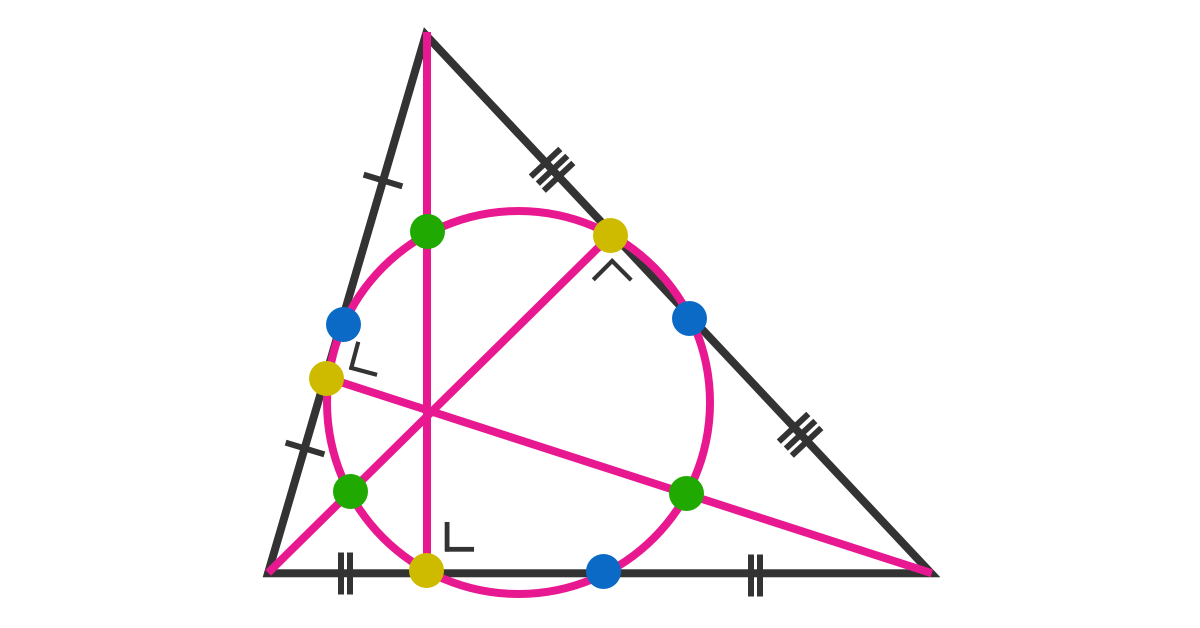
\includegraphics[width=0.9\textwidth]{obrazky-figures/NinePointCircle.png}
	\caption{Kružnica deviatich bodov. Modré body označujú stredy strán, žlté body označujú päty výšok a zelené sú stredy medzi vrcholmi a priesečníkom výšok\cite{katz_prakash_khim}}
	\label{fig:TriangleCenters_ninePoints}
\end{figure}



\subsection*{Stred objektu}
%https://www.gamedev.net/forums/topic/468405-center-of-a-3d-object/

Rovnako ako pri 2D objektoch, aj u~3D objektoch je viacero variant získania stredu objektu. Zvolil som dve metódy a to metódu ohraničujúceho kvádra a metódu priemerného stredu všetkých bodov.


\subsubsection{Stred pomocou ohraničujúceho kvádra}
Pri tejto metóde sa prejdú všetky body a zoberie sa maximálna a minimálna hodnota v~osiach X, Y a Z. Takto dostaneme ohraničujúci kváder (Bounding box) a ako výsledný bod sa zoberie stred tohto kvádra.
		
\begin{figure}[H]
	\centering
%	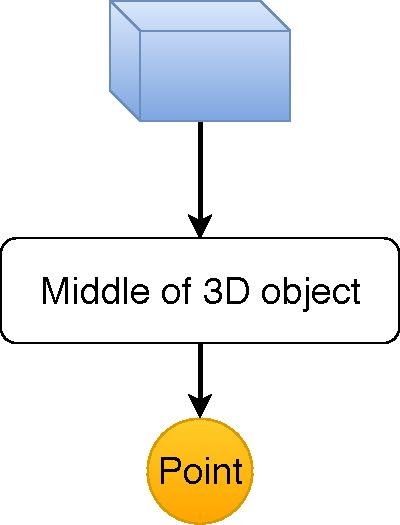
\includegraphics[height=0.3\textwidth]{obrazky-figures/Diagram/Point/DP Navrh operacii-0D - PointMiddle of 3D object.pdf}
	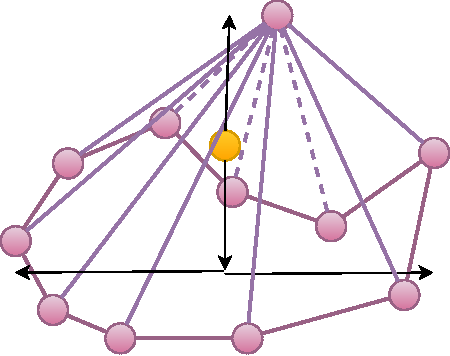
\includegraphics[height=0.3\textwidth]{obrazky-figures/Diagram/Draw/1Points/DP Navrh operacii-0D - PointMiddle of 3D object.pdf}
	\caption{Stred ohraničujúceho kvádra}
	\label{fig:PointMiddle of 3D object}
\end{figure}

\subsubsection{Priemer všetkých bodov} 
Pri tejto operácii sa sčítajú koordináty všetkých bodov. To vytvorí tri veľké čísla, ktoré sa následne vydelia počtom bodov.


% \begin{figure}[H]
% 	\centering
% %	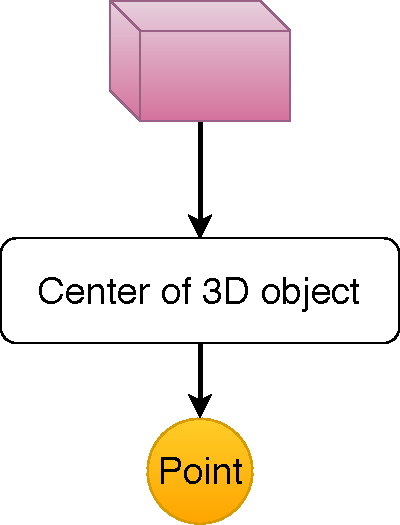
\includegraphics[height=0.3\textwidth]{obrazky-figures/Diagram/Point/DP Navrh operacii-0D - PointCenter of 3D object.pdf}
% 	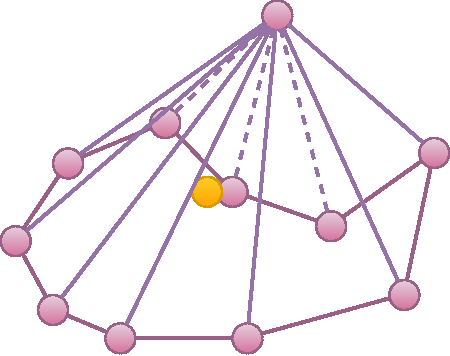
\includegraphics[height=0.3\textwidth]{obrazky-figures/Diagram/Draw/1Points/DP Navrh operacii-0D - PointCenter of 3D object.pdf}
% 	\caption{Priemerný všetkých bodov}
% 	\label{fig:1}
% \end{figure}








\section{Úsečky}
Úsečka je časť priamky medzi dvoma koncovými bodmi. Aby bolo možné používať v~geometrických operáciách smerový vektor z~úsečky, môžeme tieto body označiť ako počiatočný a koncový, ako je zobrazené na obrázku \ref{fig:Navrh operacii-1D - Line}. 
%Úsečka sa nachádza v mnohých operáciach ako parameter, kde zastupuje úlohu smerového vektoru.

\begin{equation}
    P = P1 + u(P2-P1)
    \label{eq:priamka}
\end{equation}. 

\begin{figure}[H]
	\centering
%	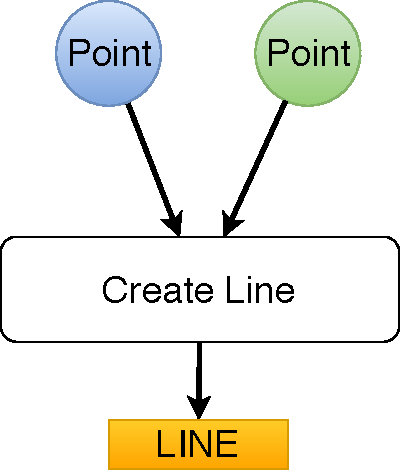
\includegraphics[height=0.3\textwidth]{obrazky-figures/Diagram/Line/DP Navrh operacii-1D - Line.pdf}
	
\includegraphics[]{obrazky-figures/Diagram/Draw/2Line/DP Navrh operacii-1D - Line.pdf}
	\caption{Zobrazenie úsečky s~počiatočným a koncovým bodom}
	\label{fig:Navrh operacii-1D - Line}
\end{figure}


\subsection*{Zmena dĺžky úsečky}
Vytvorenie úsečky so zadanou dĺžkou. Dĺžka môže byť zadaná vzdialenosťou alebo percentuálne od veľkosti zadanej úsečky. Výsledná úsečka je v~rovnakom smere a začína v~rovnakom bode ako zadaná úsečka. V~prípade ak veľkosť výslednej úsečky rovná jedna, táto geometrická operácia sa nazýva aj normalizácia.  


\begin{figure}[H]
	\centering
%	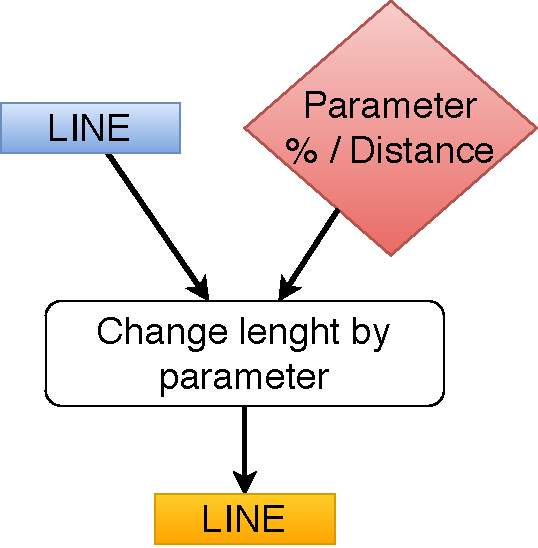
\includegraphics[height=0.3\textwidth]{obrazky-figures/Diagram/Line/DP Navrh operacii-1D - LineChangeLength.pdf}
	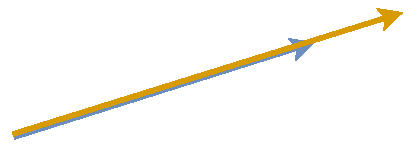
\includegraphics[]{obrazky-figures/Diagram/Draw/2Line/DP Navrh operacii-1D - LineChangeLength.pdf}
	\caption{Zmena veľkosti úsečky}
	\label{fig:LineChangeLength}
\end{figure}

\subsection*{Najkratšia úsečka medzi bodom a priamkou}\label{sec:najkratsiauseckaBP}
Priamka je definovaná dvoma bodmi, bodom $P1(x1-y1)$ a bodom $P2(x2,y2)$. 
Rovnica priamky je \ref{eq:MinlinePointLine_LineEq}.
\begin{equation}
    P = P1 + u(P2-P1)
    \label{eq:MinlinePointLine_LineEq}
\end{equation}. 

Na získanie najkratšej vzdialenosti je potrebné nájsť kolmicu od bodu $P3(x3,y3)$ na priamku. Z~toho vyplýva, že skalárny súčin medzi nimi musí byť rovný 0, tento vzťah je vidieť v~rovnici \ref{eq:MinlinePointLine_LinesEq}.

\begin{equation}
    (P3-P)\cdot(P2-P1) =0 
    \label{eq:MinlinePointLine_LinesEq}
\end{equation}
Bod P označuje najbližší bod na priamke k~bodu $P3$.

Substitúciou rovnice \ref{eq:MinlinePointLine_LineEq} do \ref{eq:MinlinePointLine_LinesEq} získame rovnicu \ref{eq:MinlinePointLine_subs}.

\begin{equation}
[P3 - P1 - u(P2-P1)] \cdot (P2 - P1) = 0
    \label{eq:MinlinePointLine_subs}
\end{equation}

Vyriešením tejto rovnice získame rovnicu \ref{eq:MinlinePointLine_subsSolved}, ktorú následne môžeme dosadiť do rovnice pre priamku \ref{eq:MinlinePointLine_LineEq} a získať pozíciu bodu $P$. Ak by sme chceli, aby sa bod vytváral iba na úsečke a nie mimo nej, bolo by potrebné testovať vzdialenosť $u$ na rozmedzie (0,1). Ak je hodnota $u$ záporná alebo väčšia ako jedna,  najbližší bod na priamke k~bodu $P3$ sa nachádza mimo zadanej úsečky. 
\begin{equation}
u= \frac
{\left (x3 -x1  \right )\left (x2-x1  \right )
+\left (y3-y1  \right )\left (y2-y1  \right )
+\left (z3-z1  \right )\left (z2-z1  \right )}
{\left \| P2-P1 \right \|^{2}}
    \label{eq:MinlinePointLine_subsSolved}
\end{equation}
Výsledná úsečka je tvorená bodmi $P$ a $P3$ \cite{bourke_Point_Line_Plane}.
%Pre získanie bodu na priamke, ktorý je najbližšie k bodu $P3$ je možné následne použiť operáciu pre získanie počiatočného bodu úsečky .



\begin{figure}[H]
	\centering
%	\includegraphics[height=0.3\textwidth]{obrazky-figures/Diagram/Line/DP Navrh operacii-1D -  LineMinPL.pdf}
	\includegraphics[height=0.3\textwidth]{obrazky-figures/Diagram/Draw/2Line/DP Navrh operacii-1D -  LineMinPL.pdf}
	\caption{Najkratšia vzdialenosť medzi úsečkou a bodom}
	\label{fig:LineMinPL}
\end{figure}

\subsection*{Najkratšia úsečka medzi dvomi priamkami}
Keďže v~trojrozmernom priestore často nenastáva pretnutie dvoch úsečiek v~jednom bode, je práve najkratšia úsečka medzi dvoma priamkami používaná ako priesečník priamok v~trojrozmernom priestore.


Hľadáme najkratšiu úsečku s~bodmi $P_a$ a $P_b$, kde $P_a$ leží na priamke definovanou bodmi $P_1$ a $P_2$, a $P_b$ leží na priamke, ktorá je definovaná bodmi $P_3$ a $P_4$.

Pre bod $P_a$ môžeme napísať rovnicu  \ref{eq:MinlineLL_Pa}.
\begin{equation}
P_a=P_1 + u_a(P_2-P_1)
    \label{eq:MinlineLL_Pa}
\end{equation}
Podobne pre bod $P_b$ rovnicu \ref{eq:MinlineLL_Pb}.
\begin{equation}
P_b=P_3 + u_b(P_4-P_3)
    \label{eq:MinlineLL_Pb}
\end{equation}
Pri hľadaní najkratšej úsečky medzi týmito priamkami si stačí uvedomiť, že najkratšia úsečka bude na tieto priamky kolmá, čo nám umožňuje zapísať následovné rovnice  \ref{eq:MinlineLL_dotab}.
\begin{equation}
\begin{aligned}
(P_a-P_b) \cdot (P_2-P_1) =0\\
(P_a-P_b) \cdot (P_4-P_3) =0
\end{aligned}
    \label{eq:MinlineLL_dotab}
\end{equation}
Po doplnení  $P_a$ a $P_b$ do týchto rovníc získame rovnice \ref{eq:MinlineLL_dotabExp}.
\begin{equation}
\begin{aligned}
((P_1 + u_a(P_2-P_1))-(P_3 + u_b(P_4-P_3))) \cdot (P_2-P_1) =0\\
((P_1 + u_a(P_2-P_1))-(P_3 + u_b(P_4-P_3))) \cdot (P_4-P_3) =0
\end{aligned}
    \label{eq:MinlineLL_dotabExp}
\end{equation}
Keďže by tieto rovnice boli veľmi rozsiahle, je vhodné si pre riešenie tejto rovnice definovať nasledovnú substitúciu \ref{eq:MinlineLL_subsdmnop}.
\begin{equation}
d_{mnop}=(x_m - x_n)(x_o-x_p)+(y_m - y_n)(y_o-y_p)+(z_m - z_n)(z_o-z_p)
    \label{eq:MinlineLL_subsdmnop}
\end{equation}
Pomocou tejto substitúcie sa dajú rovnice \ref{eq:MinlineLL_dotabExp} zapísať v~nasledovne \ref{eq:MinlineLL_dotabExpshort}.
\begin{equation}
\begin{aligned}
d_{1321} + u_a d_{2121} - u_b d_{4321} = 0\\
d_{1343} + u_a d_{2143} - u_b d_{4343} = 0
\end{aligned}
    \label{eq:MinlineLL_dotabExpshort}
\end{equation}
Vyriešením týchto rovníc pre $u_a$ získame rovnicu \ref{eq:MinlineLL_dotabExpshortSolving}.
\begin{equation}
 u_a= \frac
 {d_{1343} d_{4321} - d_{1321} d_{4343} }
 {d_{2121} d_{4343} - d_{2143} d_{2143} }
    \label{eq:MinlineLL_dotabExpshortSolving}
\end{equation}
Keď už poznáme $u_a$, pomocou dosadenia do rovnice \ref{eq:MinlineLL_dotabExpshortSolved_ub} získame $u_b$ \cite{bourke_Point_Line_Plane}.
\begin{equation}
\begin{aligned}
u_b  = \frac{d_{1321} + u_a d_{2121}}{d_{4321}}
\end{aligned}
    \label{eq:MinlineLL_dotabExpshortSolved_ub}
\end{equation}



\begin{figure}[H]
	\centering
%	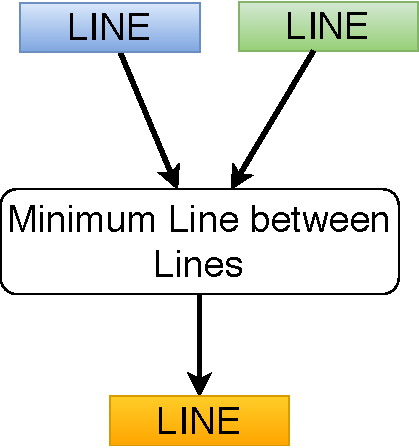
\includegraphics[height=0.3\textwidth]{obrazky-figures/Diagram/Line/DP Navrh operacii-1D - LineMinLL.pdf}
	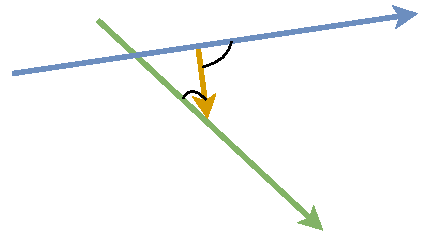
\includegraphics[height=0.3\textwidth]{obrazky-figures/Diagram/Draw/2Line/DP Navrh operacii-1D - LineMinLL.pdf}
	\caption{Najkratšia vzdialenosť medzi dvomi úsečkami}
	\label{fig:LineMinLL}
\end{figure}


\subsection*{Najkratšia úsečka medzi plochou a bodom}


Rovina je definovaná pomocou normáli $\overrightarrow{N}=(A, B, C)$ a bodom na nej ležiacom $P_a=(x_a,y_a,z_a)$.
Hľadaná úsečka má rovnaký smer ako normála plochy.
Vzdialenosť medzi touto rovinou a bodom $P_b=(x_b,y_b,z_b)$ dostaneme pomocou vzorca \ref{eq:minlineSP}, kde premietneme vektor medzi bodom $P_b$ a bodom $P_a$ na normálu roviny $\overrightarrow{N}$ pomocou skalárneho súčinu. 
\begin{equation}
 distance = (P_b - P_a) \cdot \overrightarrow{N}
    \label{eq:minlineSP}
\end{equation}

Bod $P$ získame vynásobením vektora $\overrightarrow{N}$ touto vzdialenosťou a následným odčítaním od bodu $P_b$ \ref{eq:minlineSP_P}.
\begin{equation}
 P = P_b - (\overrightarrow{N} * distance)
    \label{eq:minlineSP_P}
\end{equation}

Výsledná úsečka má počiatočný bod na ploche a koncový bod $P_b$ \cite{bourke_Point_Line_Plane}.

%Každý bod $P=(x,y,z)$ leží na rovine, ak splňuje \ref{eq:rovnicaPlochySP}.
%\begin{equation}
%Ax+By+Cz+D = 0
%    \label{eq:rovnicaPlochySP}
%\end{equation}




\begin{figure}[H]
	\centering
%	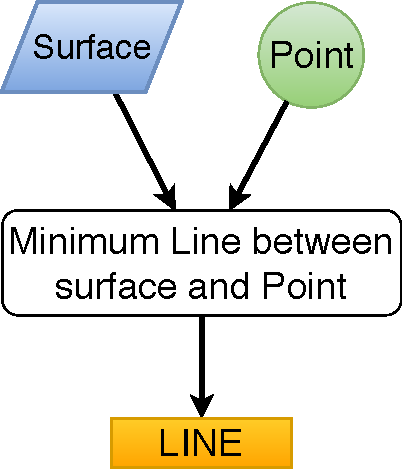
\includegraphics[height=0.3\textwidth]{obrazky-figures/Diagram/Line/DP Navrh operacii-1D - LineMinSP.pdf}
	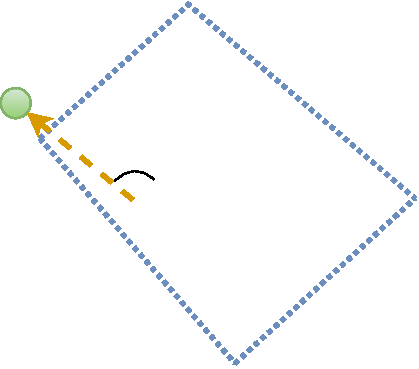
\includegraphics[height=0.3\textwidth]{obrazky-figures/Diagram/Draw/2Line/DP Navrh operacii-1D - LineMinSP.pdf}
	\caption{Najkratšia vzdialenosť medzi plochou a bodom}
	\label{fig:LineMinSP}
\end{figure}


\subsection*{Vektorový súčin}\label{subsec:crossproduct}
Vektorový súčin (cross product) vytvára úsečku, ktorá je kolmá na dané úsečky (priamky). Zadané úsečky sa najprv prevedú na vektory ($koncov\acute{y}\_bod - za\check{c}iato\check{c}n\acute{y}\_bod$).
Veľkosť úsečky závisí od veľkosti zadaných úsečiek a od uhla, ktorý zvierajú. 

\begin{equation}
 L_1 \times L_2 =  \{
 y_{l1} z_{l2} + y_{l2} z_{l1} ,
 z_{l1} x_{l2} + z_{l2} x_{l1} ,
 x_{l1} y_{l2} + x_{l2} y_{l1}\}
    \label{eq:cross}
\end{equation}


\begin{figure}[H]
	\centering
%	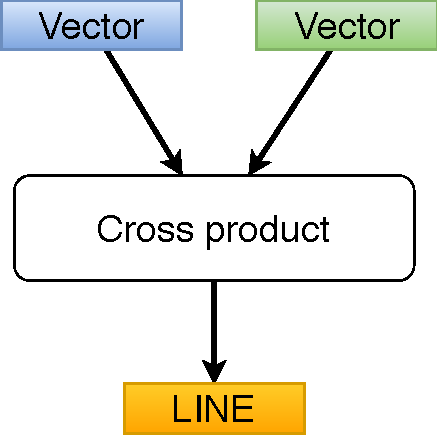
\includegraphics[height=0.3\textwidth]{obrazky-figures/Diagram/Line/DP Navrh operacii-1D - LineCross.pdf}
	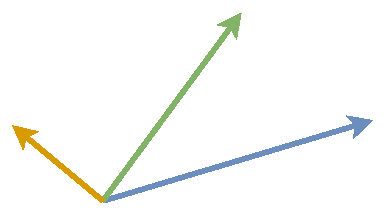
\includegraphics[height=0.3\textwidth]{obrazky-figures/Diagram/Draw/2Line/DP Navrh operacii-1D - LineCross.pdf}
	\caption{Vektorový súčin}
	\label{fig:LineCross}
\end{figure}

Táto operácia sa často používa aj v~počítačovej grafike, kde sa používa pre výpočet normály plošných útvarov. Výsledný vektor sa musí normalizovať, teda vydeliť jeho dĺžkou.
% \subsection*{Normála roviny}
% Normála plochy sa pri väčšine plošných objektov predvypočítava už pri vytváraní. Ak objekt nebol vytváraný už priamo so zadanou normálou, je potrebné ju vypočítať. Výpočet normály sa robí pomocou vektorového súčinu \ref{subsec:crossproduct}, ktorého výsledný vektor je potrebné normalizovať, teda vydeliť jeho dĺžkou.



% \subsection*{Presun úsečky}
% Táto operácia nepremiestňuje zadanú úsečku ale vytvára úsečku v rovnakom smere a rovnakej dĺžke ako zadaná úsečka $L$, ale počiatočný bod bude na pozícii zadaného bodu $P$. 
% Koncový bod úsečky $P2$ získame pomocou vzorca \ref{eq:LineReloc}. 

% \begin{equation}
%     P2 = P + (P_{2L}-P_{1L})
%     \label{eq:LineReloc}
% \end{equation}




% \begin{figure}[H]
% 	\centering
% %	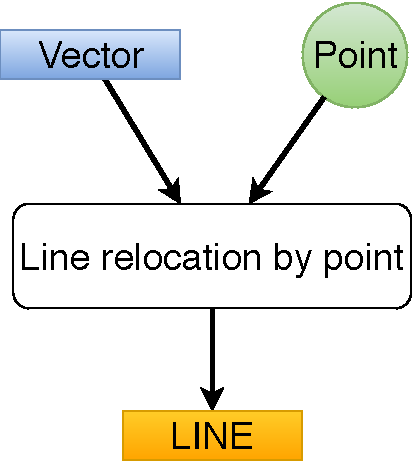
\includegraphics[height=0.3\textwidth]{obrazky-figures/Diagram/Line/DP Navrh operacii-1D - LineRelocation.pdf}
% 	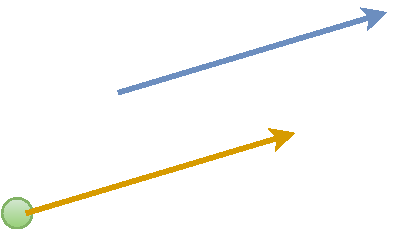
\includegraphics[height=0.3\textwidth]{obrazky-figures/Diagram/Draw/2Line/DP Navrh operacii-1D - LineRelocation.pdf}
% 	\caption{Presun úsečky}
% 	\label{fig:1}
% \end{figure}

\section{Plošné objekty}


\subsection*{Kruh}
Je viac metód ako zadávať kruh. Základným spôsobom pre vytvorenie kruhu je zadanie stredového bodu a priemeru. Keďže chceme aby bol kruh v~trojrozmernom priestore, je potrebné zadať aj normálu. 

Ďalším spôsobom je zadanie troch bodov, kde jeden z~bodov označuje stred kruhu, druhý bod leží na obvode kruhu a tretí bod ležiaci na ploche kruhu tak, aby nebol s~ostatnými bodmi na jednej priamke, označuje natočenie kruhu.

\begin{figure}[H]
	\centering
	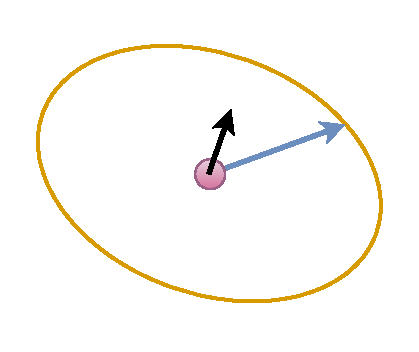
\includegraphics[height=0.3\textwidth]{obrazky-figures/Diagram/Draw/3Plane/DP Navrh operacii-2D - SurfaceCreate Circle.pdf}
	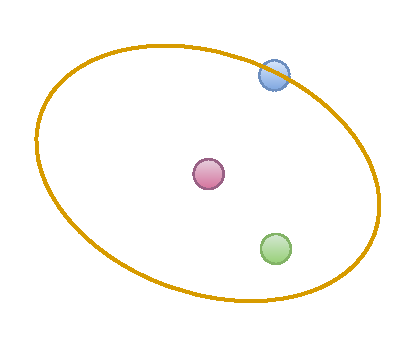
\includegraphics[height=0.3\textwidth]{obrazky-figures/Diagram/Draw/3Plane/DP Navrh operacii-2D - SurfaceCreate Circle2.pdf}
	\caption{Vľavo je kruh pomocou priemeru a normály a v~pravo je kruh tvorený troma bodmi, kde jeden bod udáva stred a pomocou ďalších dvoch bodov sa určí priemer a smer normály}
	\label{fig:SurfaceCreate Circle2}
\end{figure}

Alternatívne môžeme vyjadriť kruh pomocou opísanej (Circumscribed) alebo vpísanej (Inscribed) kružnice trojuholníka (obrázok \ref{fig:SurfaceInscribed Circumscribed Circle}). Postup pre nájdenie stredu opísanej a vpísanej kružnice trojuholníka je v~časti \ref{sec:TriangleCenter}.



\begin{figure}[H]
	\centering
	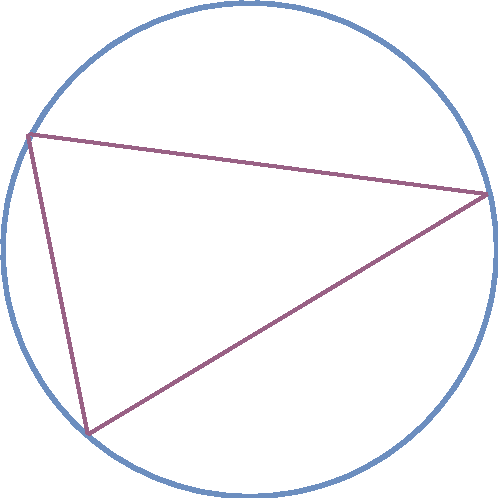
\includegraphics[height=0.3\textwidth]{obrazky-figures/Diagram/Draw/3Plane/DP Navrh operacii-2D - SurfaceCircumscribed Circle.pdf}
	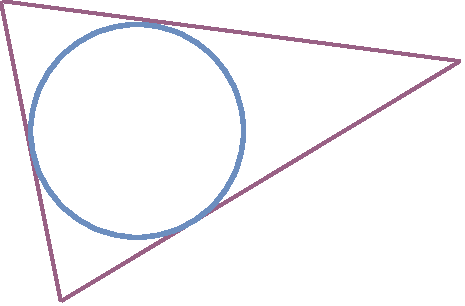
\includegraphics[height=0.3\textwidth]{obrazky-figures/Diagram/Draw/3Plane/DP Navrh operacii-2D - SurfaceInscribed Circle.pdf}
	\caption{Opísaná a vpísaná kružnica trojuholníka}
	\label{fig:SurfaceInscribed Circumscribed Circle}
\end{figure}



\subsection*{Obdĺžnik}
Často používaným geometrickým objektom v~grafike je aj obdĺžnik. Základnými parametrami obdĺžnikov je výška a šírka. Ďalším parametrom je často aj natočenie okolo normály. Keďže sa zaoberáme objektmi v~trojrozmernom priestore, obdĺžnik musí definovať aj normála, ako je vidieť na obrázku \ref{fig:SurfaceCreate Rectangle}. 


\begin{figure}[H]
	\centering

	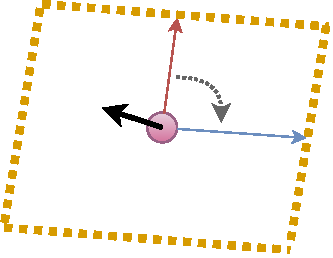
\includegraphics[height=0.3\textwidth]{obrazky-figures/Diagram/Draw/3Plane/DP Navrh operacii-2D - SurfaceCreate Rectangle.pdf}
	\caption{Obdĺžnik}
	\label{fig:SurfaceCreate Rectangle}
\end{figure}



\subsection*{Polygón}
Keďže v~reálnom svete nie sú základom objektov len dokonalé objekty ako kruh, trojuholník alebo štvorec, zvolil som pre túto prácu aj tvorbu polygónov. Polygóny pozostávajú z~množiny bodov a množinou hrán, ktoré tieto body spájajú a vytvárajú obvod polygónu. Keďže polygón je plošný útvar, musí byť tvorený minimálne 3 bodmi. Táto operácia má ako jediná premenlivý počet bodov. 

Všetky primitívne objekty, ako štvorec, kruh alebo trojuholník, sú konvexné, teda všetky vnútorné uhly sú menšie alebo rovné 90 stupňov. Proces triangulácie je v~tomto prípade veľmi jednoduchý. Stačí spojiť jeden ľubovoľný bod so všetkými ostatnými bodmi. Pri zadávaní polygónov pomocou bodov sa ale môže stať, že niektorý vnútorný uhol polygónu bude tupý, teda väčší ako 90 stupňov. Klasická metóda triangulácie teda nepostačuje a je potrebné vybrať niektorú inú metódu, napríklad \textit{Ear clipping method}.













































\section{Objemové objekty}
Medzi základné geometrické objemové telesá patrí guľa, kváder, valec, a ihlan. Nad týmito geometrickými telesami je možné vykonávať rôzne geometrické operácie.


% \subsection{Valec}


% \begin{figure}[H]
% 	\centering
% 	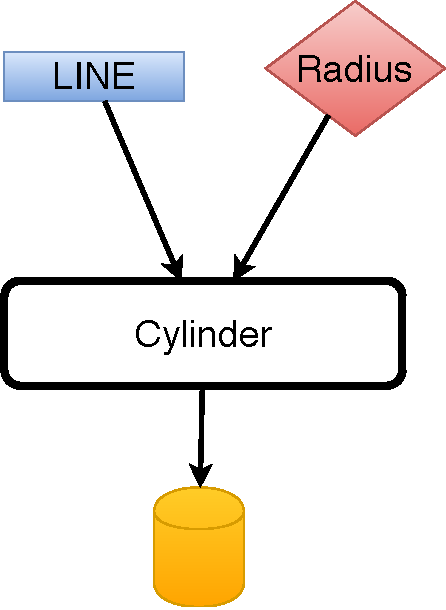
\includegraphics[height=0.3\textwidth]{obrazky-figures/Diagram/Volumetric/DP Navrh operacii-3D - ObjectsCylinder.pdf}
% 	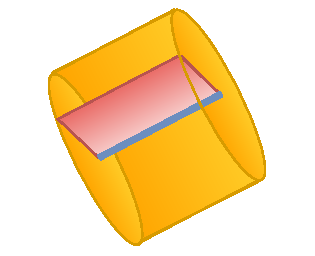
\includegraphics[height=0.3\textwidth]{obrazky-figures/Diagram/Draw/4Object/DP Navrh operacii-3D - ObjectsCylinder.pdf}
% 	\caption{Valec}
% 	\label{fig:ObjectsCylinder}
% \end{figure}

% \subsection*{Guľa}


% \subsection*{Ihlan}


\begin{figure}[H]
	\centering
% 	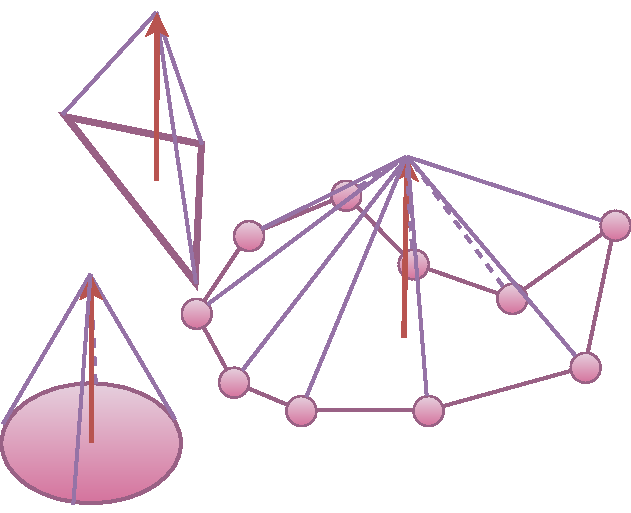
\includegraphics[height=0.3\textwidth]{obrazky-figures/Diagram/Draw/4Object/DP Navrh operacii-3D - ObjectsCreate Pyramid by distance from center.pdf}
	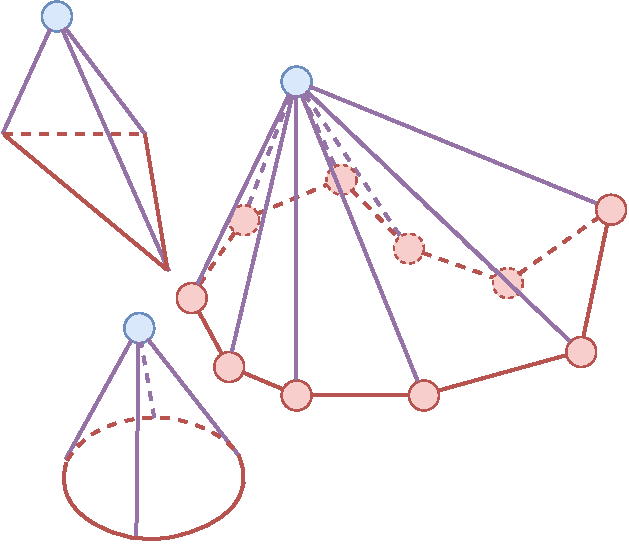
\includegraphics[height=0.3\textwidth]{obrazky-figures/Diagram/Draw/4Object/DP Navrh operacii-3D - ObjectsCreate Pyramid.pdf}
	\caption{Ihlany s~rôznymi základmi.}
	\label{fig:ObjectsCreate Pyramid}
\end{figure}


\subsection*{Extrudovanie} 
Natiahne plochu do priestoru v~smere normály, čím získa na objeme. Pomocou tejto operácie sa dá vytvoriť aj napríklad kváder alebo valec, ak je základ štvorcového, respektívne kruhového tvaru. Táto operácia je zobrazená na obrázku \ref{fig:ObjectsExtrude}, kde je fialovým zobrazená počiatočná plocha a žltým je zobrazená extrudácia. Extrudáciu je možné spraviť tak, že sa vytvorí kópia zadanej plochy a posunie sa o~zadaný offset. Tieto dve plochy sa následne prepoja. Častou modifikáciou je extrudovanie po krivke a/alebo postupná zmena veľkosti. 




\begin{figure}[H]
	\centering
% 	\includegraphics[height=0.3\textwidth]{obrazky-figures/Diagram/Volumetric/DP Navrh operacii-3D - ObjectsExtrude.pdf}
	\includegraphics[height=0.3\textwidth]{obrazky-figures/Diagram/Draw/4Object/DP Navrh operacii-3D - ObjectsExtrude.pdf}
	\caption{Extrudovanie}
	\label{fig:ObjectsExtrude}
\end{figure}


% \subsection{Zagulatená plocha}


% \begin{figure}[H]
% 	\centering
% 	\includegraphics[height=0.3\textwidth]{obrazky-figures/Diagram/Volumetric/DP Navrh operacii-3D - ObjectsSpherical curved surface.pdf}
% 	\includegraphics[height=0.3\textwidth]{obrazky-figures/Diagram/Draw/4Object/DP Navrh operacii-3D - ObjectsSpherical curved surface.pdf}
% 	\caption{Zagulatenie plochy}
% 	\label{fig:ObjectsSpherical curved surface}
% \end{figure}





\subsection*{Booleovské operácie nad objemovými telesami}
\label{sec:libigl}
Pre vytvorenie zložitejších objektov je potrebné jednoduché objekty skladať pomocou booleovských operácií ako zjednotenie (union), prienik (intersection) a rozdiel medzi množinami (minus). Tieto operácie sú zobrazené aj na obrázku \ref{fig:BooleanOperation}, kde tvoria CSG (constructive solid geometry) strom. Keďže sú tieto operácie náročné na spracovanie, rozhodol som sa využiť niektorú z~voľne dostupných knižníc. Našiel som niekoľko dostupných knižníc, ktoré by sa dali použiť. Jednou z~nich je \texttt{libigl}\cite{libigl}.
%https://stackoverflow.com/questions/24694845/c-library-for-mesh-to-mesh-intersection-what-is-available
%https://libigl.github.io/tutorial/#boolean-operations-on-meshes

Knižnica libigl je používaná aj veľkými spoločnosťami ako je Activision, EA, Adobe, Google, Epic Games, Microsoft, Pixar, UBISOFT a ďalšie. Táto knižnica je distribuovaná pod licenciou Mozilla Public License (MPL).
Obľúbená je hlavne pre svoju jednoduchosť. Pre tvorbu booleovských operácií nad mesh stačí zavolať funkciu \texttt{mesh\_boolean}.
Táto funkcia pracuje s~bodmi (V) a trojuholníkmi (F). Na výpočet zjednotenia (typ \\ \texttt{MESH\_BOOLEAN\_TYPE\_UNION}) pre mesh $A=(VA,FA)$ a mesh $B=(VB,FB)$ je nasledovná funkcia. Výsledok tejto funkcie sa uloží do mesh $C=(VC,FC)$,

\begin{lstlisting}
igl::copyleft::cgal::mesh_boolean(VA,FA,VB,FB,MESH_BOOLEAN_TYPE_UNION,VC,FC);
\end{lstlisting}

\begin{figure}[H]
	\centering
	\includegraphics[width=\textwidth]{obrazky-figures/cube-sphere-cylinders-csg-tree.jpg}
	\caption{Skladanie objektov pomocou booleovských operácii}
	\label{fig:BooleanOperation}
\end{figure}





















































% \chapter{\todo{treba zmenit}}
% Geometrické operácie sa delia na 4 typy podľa toho, aký typ objektu sa dá pomocou nich vytvoriť. Sú to operácie bodové, úsečkové, plošné a priestorové. Na vytváranie zložitejších objektov je potrebné využívať jednoduchšie geometrické objekty. 

% Všetky geometrické operácie sa dajú zapisovať pomocou textovej podoby. Tento textový zápis operácií je taktiež uvedený pri jednotlivých operáciach nižšie. 
% Textová podoba geometrickej operácie sa začína názvom použitej geometrickej operácie a parametrami uvedenými v zátvorkách ( a ), oddelenými znakom \texttt{','}.  U jednotlivých parametrov sa medzery na začiatku a konci ignorujú.

% Pri parametroch typu $Float$ sa požaduje desatinné číslo, pri ostatných parametroch je potrebné uviesť názov existujúceho objektu, ktorý je rovnakého typu alebo podtypu aký je vyžadovaný. Požadované parametre pre jednotlivé geometrické operácie sú uvedené nižšie. 

% Parametrom typu $Float$ je možné vytvoriť názov, pomocou ktorého sa bude dať na daný parameter neskôr pristupovať. 
% Tento názov sa zadáva za hodnotou parametra oddelený znakom \texttt{';'}.

% Jednotlivé operácie sa oddeľujú bodkočiarkou \texttt{';'}. 
% Táto textová podoba geometrických operácií sa používa aj pre uloženie do súboru a jeho neskoršie načítanie. 

% Pre predstavu ako sa jednotlivé objekty vytvárajú uvádzam príklad pre vytvorenie ihlana s kruhovou podstavou s polomerom 5 a výškou 10:
% \begin{itemize}
%     \item Na vytvorenie ihlana je potrebné najprv vytvoriť bod na pozícii XYZ, napr. $\left [ 1, 2, 3 \right ]$, ktorý bude slúžiť ako stred kruhovej podstavy.
% 	\begin{lstlisting}
% 	Point(bod podstavy, 1, 2, 3 ,0);
% 	\end{lstlisting}
% 	\item Na vytvorenie kruhu (podstavy ihlana) je potrebný polomer a normála. Ako normálu, je možné využiť smer ľubovolnej úsečky, ale keďže zatiaľ žiadnu úsečku vytvorenú nemáme, je potrebné ju vytvoriť. Úsečka sa skladá z dvoch bodov a to počiatočného a koncového. Ako normála, sa použije normalizovaný vektor medzi bodom počiatočným a koncovým \ref{eq:normalizacia_usecky}.

% 	\begin{equation}
% 		\overrightarrow{normal\_vector}=
% 		\frac{end\_point - begin\_point}{
% 		\left \|  end\_point - begin\_point \right \|}
% 	\label{eq:normalizacia_usecky}
% 	\end{equation}

% 	\begin{lstlisting}
% 	Point(počiatočný bod, 0, 0, 0, 0);
% 	Point(koncový bod, 1, 1, 1, 0);
% 	Line(normála, počiatočný bod, koncový bod, 0);
% 	\end{lstlisting}
% 	\item Keď už je normála vytvorená, je možné vytvoriť kruh s polomerom 5.
% 	\begin{lstlisting}
% 	Circle(podstava, bod podstavy, 5, normála, 0) 
% 	\end{lstlisting}
% 	\item Ostáva vytvoriť samotný ihlan s výškou 10.
% 	\begin{lstlisting}
% 	Pyramid(ihlan s kruhovou podstavou, podstava, 10, 1)
% 	\end{lstlisting}
% \end{itemize}

% \todo{ako vyzerá tento sled operácií pomocou graphviz a v 3D}

% Ďalej nasleduje výpis podporovaných geometrických operácií, kde pri každej operácií sa nachádza jednoduchý popis, formát zápisu tejto operácie a grafové zobrazenie vytvorenia tejto operácie.


% \section{Bodové operácie}
% Bodové operácie sú operácie, ktorých výstupom je bod.
% \subsection{Bod}
% Základná stavebná jednotka každého objektu. Na vytvorenie bodu je potrebné zadať jeho pozíciu v osiach X, Y a Z. Bod môže byť zadaný buď v absolútnej alebo v relatívnej pozícii, kedy je jeho pozícia závislá na polohe iného bodu.
% \begin{lstlisting}
%     Point(string name, float X, float Y, float Z,float visibility) 
%     Point(string name, float X, float Y, float Z,Point Parent,
%         float visibility)
% \end{lstlisting}

% \begin{figure}[H]
% 	\centering
% 	\includegraphics[height=0.3\textwidth]{obrazky-figures/Diagram/Point/DP Navrh operacii-0D - Point.pdf}
% 	\includegraphics[height=0.3\textwidth]{obrazky-figures/Diagram/Draw/1Points/DP Navrh operacii-0D - Point.pdf}
% 	\caption{Vytvorenie bodu na absolútnej pozícii}
% 	\label{fig:1}
% \end{figure}
% \begin{figure}[H]
% 	\centering
% 	\includegraphics[height=0.3\textwidth]{obrazky-figures/Diagram/Point/DP Navrh operacii-0D - Point2.pdf}
% 	\includegraphics[height=0.3\textwidth]{obrazky-figures/Diagram/Draw/1Points/DP Navrh operacii-0D - PointRelative.pdf}
% 	\caption{Vytvorenie bodu na relatívnej pozícii od iného bodu}
% 	\label{fig:1}
% \end{figure}

% \subsection{Lineárna interpolácia}
% Výsledná pozícia bodu závisí od zadanej vzdia\-le\-nos\-ti od počiatočného bodu. Táto vzdia\-le\-nosť môže byť zadaná dĺžkou alebo percentuálne, kde 50\% vytvorí bod uprostred počiatočného a koncového bodu. 
% Keďže percentá sa zadávajú tiež vo formáte desatinného čísla ($Float$), bolo potrebné tieto operácie rozlíšiť. Pre zadanie vzdialenosti podľa dĺžky, sa zadáva operácia \texttt{LinearInterpolationDist}, 
% pre percentuálnu vzdialenosť je operácia \texttt{LinearInterpolationPerc}.
% \begin{lstlisting}
%     LinearInterpolationDist(string name, Point fromPoint, Point toPoint,
%         float distance, float visibility)
%     LinearInterpolationPerc(string name, Point fromPoint, Point toPoint,
%         float percentage, float visibility)
% \end{lstlisting}


% \begin{figure}[H]
% 	\centering
% 	\subfloat{\includegraphics[height=0.3\textwidth]{obrazky-figures/Diagram/Point/DP Navrh operacii-0D - Point Linear interpolation.pdf}}
% 	\subfloat{\includegraphics[]{obrazky-figures/Diagram/Draw/1Points/DP Navrh operacii-0D - PointLinearInterpolation.pdf}}
% 	\caption{Lineárna interpolácia}
% 	\label{fig:1}
% \end{figure}

% Ak je zadaná vzdialenosť pomocou dĺžky, použije sa vzorec \ref{eq:LiearnInterpolation}. Pri percentuálnej vzdialenosti sa použije obdobný vzorec, ale vektor medzi bodmi bod1 a bod2 sa nenormalizuje.
% \begin{equation}
%     bod = bod1 + norm(bod2 - bod1) * vzdialenos\check{t};
% 	\label{eq:LiearnInterpolation}
% \end{equation}


% \subsection{Priesečník plochy a úsečky}
% http://paulbourke.net/geometry/pointlineplane/

% Pri tejto operácii sa používa ľubovolný plošný objekt ako rovina a úsečka ako priamka. Táto geometrická operácia vytvorí bod v mieste, kde sa priamka pretína s rovinou. 


% \begin{figure}[H]
% 	\centering
% 	\includegraphics[height=0.3\textwidth]{obrazky-figures/DP Navrh operacii-Intersection.pdf}
% 	\caption{Pretnutie plochy priamkou}
% 	\label{fig:1}
% \end{figure}


% Rovnica pre rovinu, ktorá je tvorená bodom \texttt{P\textsubscript{3}} nachádzajúcom sa na rovine a normálou N, sa dá zapísať ako \ref{eq:rovnicaPlochy_intersection}. 
% \begin{equation}
%     \textbf{N} \cdot (\textbf{P} - \textbf{P3}) = 0
% 	\label{eq:rovnicaPlochy_intersection}
% \end{equation}

% Rovnica pre priamku, ktorá je určená bodmi \texttt{P\textsubscript{1}} a \texttt{P\textsubscript{2}}
% \ref{eq:rovnicaPriamky_intersection}
% \begin{equation}
% 	\textup{P}=\textbf{P1}+u (\textbf{P2}-\textbf{P1})
%     \label{eq:rovnicaPriamky_intersection}
% \end{equation}
	
% Bod \texttt{P} označuje priesečník medzi rovinou a priamkou. Pomocou substitúcie získame rovnicu \ref{eq:rovnicaPriesecniku}.

% \begin{equation}
% 	\textbf{N} \cdot (\textbf{P1}+u(\textbf{P2}-\textbf{P1}))) = \textbf{N} \cdot \textbf{P3}
%     \label{eq:rovnicaPriesecniku}
% \end{equation}

% Po vyriešení tejto rovnice dostaneme rovnicu \ref{eq:rovnicaPriesecnikuSolved}. Výslednú pozíciu bodu dostaneme dosadením $u$ do rovnice pre  priamku \ref{eq:rovnicaPriamky_intersection}.
% \begin{equation}
% 	u=\frac
% {\textbf{N} \cdot (\textbf{P3}-\textbf{P1})}
% {\textbf{N} \cdot (\textbf{P2}-\textbf{P1})}
%     \label{eq:rovnicaPriesecnikuSolved}
% \end{equation}


% \begin{lstlisting}
% 	Intersection_Plane_Line(string name, Line lineName, Sufrace surfaceName,
% 	    float visibility)
% \end{lstlisting}

% Ako je vidieť na obrázku \ref{fig:GraphIntersection_Plane_Line}, pomocou tejto operácie sa vytvorí bod aj mimo zadaných objektov. Problém nastáva, ak je zadaná úsečka paralelná s plochou a teda je kolmá na normálu plochy $N$. Skalárny súčin v menovateli je potom rovný 0. V tomto prípade nieje možné nájsť priesečník.

% \begin{figure}[H]
% 	\centering
% 	\includegraphics[height=0.3\textwidth]{obrazky-figures/Diagram/Point/DP Navrh operacii-0D - PointIntersection PlaneLine.pdf}
% 	\includegraphics[height=0.3\textwidth]{obrazky-figures/Diagram/Draw/1Points/DP Navrh operacii-0D - PointIntersectionPlaneLine.pdf}
% 	\caption{Priesečník plochy a priamky.}
% 	\label{fig:GraphIntersection_Plane_Line}
% \end{figure}

% \subsection{Stred plochy}
% Existuje množstvo možností ako získať stred objektu. Do tejto práce som vybral dve, metódu minimálneho štvorca a priemer všetkých bodov. Pri týchto operáciach sa prevádza 
% zadaná plocha z trojrozmerného priestoru  do dvojrozmerného.


% \subsubsection{Minimálny štvorec}
% Pri tejto operácii sa prejdú všetky body a zistí sa maximálna a minimálna hodnota v jednotlivých osiach a výsledný bod sa nachádza uprostred nich.


% \begin{lstlisting}
% 	SurfaceCenterMinimalSquare(string name, Surface surfaceName, float visibility)
% \end{lstlisting}
% %//Create point on position of middle of entered surface
% %	//	Example:
% %	//		SurfaceMiddle(PointName, Circle)	//- Create Point on center of Circle
% %	//		SurfaceMiddle(PointName, Rectangle)	//- Create Point on middle of Rectangle
% %	//		SurfaceCenter(PointName, Shape)		//- Create Point on middle of shape 
% %	//		SurfaceMiddle(PointName, Shape)		//- Create Point on middle of shape - centroid (sum of points / count of points)

% \begin{figure}[H]
% 	\centering
% 	\includegraphics[height=0.3\textwidth]{obrazky-figures/Diagram/Point/DP Navrh operacii-0D - PointMiddle of surface.pdf}
% 	\includegraphics[height=0.3\textwidth]{obrazky-figures/Diagram/Draw/1Points/DP Navrh operacii-0D - PointMiddle of surface.pdf}
% 	\caption{Stred plochy pomocou minimálneho štvorca }
% 	\label{fig:1}
% \end{figure}



% \subsubsection{Priemer všetkých bodov}
% Nájde aritmetický priemer všetkých bodov polygónu.

% \begin{equation}
%     \frac{1}{n} \sum_{i=0}^{n} p_i   
%     \label{eq:aritPriemer}
% \end{equation}
% \begin{lstlisting}
% 	SurfaceCenterAverage(string name, Surface surfaceName, float visibility)
% \end{lstlisting}


% \begin{figure}[H]
% 	\centering
% 	\includegraphics[height=0.3\textwidth]{obrazky-figures/Diagram/Point/DP Navrh operacii-0D - PointCenter of surface.pdf}
% 	\includegraphics[height=0.3\textwidth]{obrazky-figures/Diagram/Draw/1Points/DP Navrh operacii-0D - PointCenter of surface.pdf}
% 	\caption{Stred plochy pomocou výpočtu priemeru všetkých bodov}
% 	\label{fig:1}
% \end{figure}

% \subsubsection{Stred trojuholníku}
% Pre stred trojuholníka existuje v súčastnosti, podľa encyklopédie stredov trojuholníkov, až 30 483 trojuholníkových centier \cite{http://faculty.evansville.edu/ck6/encyclopedia/ETC.html}. Tento počet každým dňom narastá. Pre porovnanie, v decembri 2004 bolo známych 3053 \cite{http://mathworld.wolfram.com/KimberlingCenter.html}. Medzi najznámejšie patria ťažisko (G), ortocentrum (H), stred vpísanej kružnice (I), opísanej kružnice (O) aj stred kružnice deviatich bodov (N). Tieto body sú zaznačené na obrázku \ref{fig:TriangleCenters}.


% \begin{figure}[H]
% 	\centering
% 	\includegraphics[width=0.9\textwidth]{obrazky-figures/Trigonometric_centres.png}
% 	\caption{Najznámejšie stredy trojuholníka sú ťažisko (G), ortocentrum (H), stred vpísanej kružnice (I), opísanej kružnice (O) aj stred kružnice deviatich bodov (N)}
% 	\label{fig:TriangleCenters}
% \end{figure}


% \paragraph{Ťažisko (Centroid)}\mbox{} \\

% Ťažisko trojuholníku sa nachádza v priesečníku troch mediánov trojuholníka. Na nájdenie jeho pozície stačí vypočítať aritmetický priemer vrcholov trojuholníka v jednotlivých osiach \ref{eq:triangleCentroid} \cite{https://brilliant.org/wiki/triangles-centroid/}.



% \begin{equation}
%     \frac{A+B+C}{3}
%     \label{eq:triangleCentroid}
% \end{equation}

% \paragraph{Stred vpísanej kružnice (Incenter)}\mbox{} \\

% Z každého bodu trojuholníka urobíme priamku tak, aby uhly na oboch stranách priam\-ky boli rovnaké. Táto priamka sa nazýva tiež bisektor \cite{https://www.tutorvista.com/math/angle-bisector-theorem}. Stred vpísanej kružnice je na priesečníku týchto priamok.




% Stred vpísanej kružnice sa dá vypočítať aj pomocou vzorca \ref{eq:Incenter} \cite{https://www.mathopenref.com/coordincenter.html}.
% \begin{equation}
% O = \frac{a\ast A+b\ast  B +c \ast C}{a + b + c}
%     \label{eq:Incenter}
% \end{equation}
% kde  $A$, $B$, $C$ sú vrcholy trojuholníka a $a$, $b$, $c$ sú dĺžky strán protiľahlých k vrcholom $A$, $B$, $C$.

% \paragraph{Stred opísanej kružnice (Circumcenter)}\mbox{} \\

% U jednotlivých strán trojuholníka zistíme stred a z tohto bodu urobíme kolmice. Kde sa tieto kolmice stretnú, vznikne stred vpísanej kružnice. Veľkosť kružnice je vzdialenosť od stredu k ľubovolnému vrcholu trojuholníka. Táto vzdialenosť je pre všetky vrcholy rovnaká.


% \paragraph{Ortocentrum (Orthocenter)}\mbox{} \\

% Ortocentrum sa nachádza na priesečníku kolmíc, ktoré prechádzajú cez protiľahlí vrchol. Tieto kolmice sa tiež nazývajú výškou trojuholníka. 
% Ak je trojuholník tupý, ortocentrum sa nachádza mimo trojuholníka, ak je trojuholník v niektorom vrchole kolmý, nachádza sa v takomto vrchole aj ortocentrum trojuholníka.

% Pre získanie pozície ortocentra zistíme aspoň dve kolmice pomocou operácie \ref{sec:najkratsiauseckaBP}. Pozícia ortocentra sa nachádza v mieste, kde sa tieto kolmice pretínajú. 


% \paragraph{Stred kružnice deviatich bodov (NinePointCenter)}\mbox{} \\

% Kružnica deviatich bodov, tiež známa ako Feuefbachova kružnica, po nemeckom matematikovi Karl Wilhelm Feuerbach, ktorý ako prvý dokázal, že sa kružnica deviatich bodov dotýka vpísanej a pripísaných kružníc \cite{NinePointTheorem} 


% \newtheorem{theorem}{Teorém}
 
% \begin{theorem}[{\cite{https://lms.umb.sk/mod/book/tool/print/index.php?id=76930&chapterid=1746} Teorém kružnice deviatich bodov}]
% Nech ABC je všeobecný trojuholník, P,Q,R nech sú päty jeho výšok, K,L,M nech sú stredy jeho strán, O nech je priesečník výšok a T,U,V nech sú postupne stredy úsečiek AO,BO,CO. Potom 9 bodov P,Q,R,K,L,M,T,U,V leží na jednej (tzv. Feuerbachovej) kružnici. \todo{Ako citovať? https://lms.umb.sk/mod/book/tool/print/index.php?id=76930&chapterid=1746}

% \end{theorem}


% \begin{figure}[H]
% 	\centering
% 	\includegraphics[width=0.9\textwidth]{obrazky-figures/NinePointCircle.png}
% 	\caption{Kružnica deviatich bodov. Modré body označujú stredy strán, žlté body označujú päty výšok a zelené sú stredy medzi vrcholmi a priesečníkom výšok}
% 	\label{fig:TriangleCenters}
% \end{figure}



% \subsection{Stred objektu}
% https://www.gamedev.net/forums/topic/468405-center-of-a-3d-object/

% Rovnako ako pri 2D objektoch, aj u 3D objektoch je viacero variant získania stredu objektu. Vybral som metódu ohraničujúceho kvádra a metódu priemerného stredu všetkých bodov.


% \subsubsection{Stred pomocou ohraničujúceho kvádra}
% Prejde všetky body a zoberie maximálnu a minimálnu hodnotu v osiach X, Y a Z. Takto dostaneme ohraničujúci kváder (Bounding box) a ako výsledný bod sa zoberie stred tohto kvádra.

% \begin{lstlisting}
% 	ObjectCenterBoundingBox(string name, Object3D ObjectName, 
% 		float visibility)
% \end{lstlisting}
		
% \begin{figure}[H]
% 	\centering
% 	\includegraphics[height=0.3\textwidth]{obrazky-figures/Diagram/Point/DP Navrh operacii-0D - PointMiddle of 3D object.pdf}
% 	\includegraphics[height=0.3\textwidth]{obrazky-figures/Diagram/Draw/1Points/DP Navrh operacii-0D - PointMiddle of 3D object.pdf}
% 	\caption{Stred ohraničujúceho kvádra}
% 	\label{fig:1}
% \end{figure}

% \subsubsection{Priemer všetkých bodov} 
% Pri tejto operácii sa spočítajú koordináty všetkých bodov. To vytvorí tri veľké čísla, ktoré sa následne vydelia počtom bodov.

% \begin{lstlisting}
% 	ObjectCenterAverage(string name, Object3D ObjectName,
% 		float visibility)
% \end{lstlisting}

% \begin{figure}[H]
% 	\centering
% 	\includegraphics[height=0.3\textwidth]{obrazky-figures/Diagram/Point/DP Navrh operacii-0D - PointCenter of 3D object.pdf}
% 	\includegraphics[height=0.3\textwidth]{obrazky-figures/Diagram/Draw/1Points/DP Navrh operacii-0D - PointCenter of 3D object.pdf}
% 	\caption{Priemerný všetkých bodov}
% 	\label{fig:1}
% \end{figure}

% \subsection{Začiatok a koniec úsečky}
% Aby sa dalo pristupovať k začiatočnému a koncovému bodu úsečky, vytvoril som operácie \texttt{LineFirstPoint} a \textt{LineSecondPoint}.
% \label{sec:begandendofline}

% \begin{lstlisting}
%     LineFirstPoint(string name, Line lineName, float visibility)
%     LineSecondPoint(string name, Line lineName, float visibility)
% \end{lstlisting}
		
		


% \begin{figure}[H]
% 	\centering
% 	\includegraphics[height=0.3\textwidth]{obrazky-figures/Diagram/Point/DP Navrh operacii-0D - PointFirst POINT of LINE.pdf}
% 	\includegraphics[height=0.3\textwidth]{obrazky-figures/Diagram/Draw/1Points/DP Navrh operacii-0D - PointFirstPointOfLine.pdf}
% 	\caption{Počiatočný bod úsečky}
% 	\label{fig:1}
% \end{figure}



% \begin{figure}[H]
% 	\centering
% 	\includegraphics[height=0.3\textwidth]{obrazky-figures/Diagram/Point/DP Navrh operacii-0D - PointSecond POINT of LINE.pdf}
% 	\includegraphics[height=0.3\textwidth]{obrazky-figures/Diagram/Draw/1Points/DP Navrh operacii-0D - PointSecondPointOfLine.pdf}
% 	\caption{Koncový bod úsečky}
% 	\label{fig:1}
% \end{figure}



	






% \section{Úsečkové operácie}
% Geometrické operácie vytvárajúce úsečky. 

% \subsection{Úsečka}
% Úsečka sa nachádza v mnohých operáciach ako parameter, kde zastupuje úlohu smerového vektoru. Každá úsečka sa začína počiatočným bodom a končí koncovým bodom. Pre získanie počiatočného a koncového bodu sú operácie \ref{sec:begandendofline}.

% \begin{lstlisting}
% 	Line(string lineName, Point počiatočný_bod, Point koncový_bod, float visibility)
% \end{lstlisting}

% \begin{figure}[H]
% 	\centering
% 	\includegraphics[height=0.3\textwidth]{obrazky-figures/Diagram/Line/DP Navrh operacii-1D - Line.pdf}
% 	\includegraphics[]{obrazky-figures/Diagram/Draw/2Line/DP Navrh operacii-1D - Line.pdf}
% 	\caption{Vytvorenie úsečky pomocou bodu počiatočného a bodu koncového}
% 	\label{fig:1}
% \end{figure}

% \subsection{Normalizovanie veľkosti úsečky}
% Táto operácia vytvorí úsečku s dĺžkou 1 v rovnakom smere ako pôvodná a s rovnakým počiatočným bodom.
% \begin{lstlisting}
% 	LineNormalize(string lineName, Line l, float visibility)
% \end{lstlisting}

% \begin{figure}[H]
% 	\centering
% 	\includegraphics[height=0.3\textwidth]{obrazky-figures/Diagram/Line/DP Navrh operacii-1D - LineNormalize.pdf}
% 	\includegraphics[]{obrazky-figures/Diagram/Draw/2Line/DP Navrh operacii-1D - LineNormalize.pdf}
% 	\caption{Normalizácia veľkosti úsečky}
% 	\label{fig:1}
% \end{figure}

% \subsection{Zmena dĺžky úsečky}
% Vytvorenie úsečky so zadanou dĺžkou. Dĺžka môže byť zadaná vzdialenosťou alebo percentuálne od veľkosti zadanej úsečky. Výsledná úsečka je v rovnakom smere a začína v rovnakom bode ako zadaná úsečka. V prípade ak je veľkosť výslednej úsečky 
% \begin{lstlisting}
% 	LineChangeLengthDist(string lineName, Line l, float distance, 
% 	    float visibility)
% 	LineChangeLengthPerc(string lineName, Line l, float percent, 
% 	    float visibility) 
% \end{lstlisting}%//percent = (0;100>

% \begin{figure}[H]
% 	\centering
% 	\includegraphics[height=0.3\textwidth]{obrazky-figures/Diagram/Line/DP Navrh operacii-1D - LineChangeLength.pdf}
% 	\includegraphics[]{obrazky-figures/Diagram/Draw/2Line/DP Navrh operacii-1D - LineChangeLength.pdf}
% 	\caption{Zmena veľkosti úsečky}
% 	\label{fig:1}
% \end{figure}

% \subsection{Najkratšia úsečka medzi bodom a priamkou}\label{sec:najkratsiauseckaBP}
% Priamka je definovaná dvoma bodmi, bodom $P1(x1-y1)$ a bodom $P2(x2,y2)$. 
% Rovnica priamky je 
% \begin{equation}
%     P = P1 + u(P2-P1)
%     \label{eq:MinlinePointLine_LineEq}
% \end{equation}. 

% Na získanie najkratšej vzdialenosti je potrebné nájsť kolmicu od bodu $P3(x3,y3)$ na priamku. Z toho vyplýva, že skalárny súčin medzi nimi musí byť rovný 0, tento vzťah je vidieť v rovnici \ref{eq:MinlinePointLine_LinesEq}.

% \begin{equation}
%     (P3-P)\cdot(P2-P1) =0 
%     \label{eq:MinlinePointLine_LinesEq}
% \end{equation}
% Bod P označuje najbližší bod na priamke k bodu $P3$.

% Substitúciou rovníc \ref{eq:MinlinePointLine_LineEq} a \ref{eq:MinlinePointLine_LinesEq} získame rovnicu \ref{eq:MinlinePointLine_subs}.

% \begin{equation}
% [P3 - P1 - u(P2-P1)] \cdot (P2 - P1) = 0
%     \label{eq:MinlinePointLine_subs}
% \end{equation}

% Vyriešením tejto rovnice získame rovnicu \ref{eq:MinlinePointLine_subsSolved}, ktorú následne môžeme dosadiť do rovnice pre priamku \ref{eq:MinlinePointLine_LineEq} a získať pozíciu bodu $P$. Ak by sme chceli, aby sa bod vytváral iba na úsečke a nie mimo nej, bolo by potrebné testovať vzdialenosť $u$ na rozmedzie (0,1). Ak je hodnota $u$ záporná alebo väčšia ako jedna,  najbližší bod na priamke k bodu $P3$ sa nachádza mimo zadanej úsečky. 
% \begin{equation}
% u= \frac
% {\left (x3 -x1  \right )\left (x2-x1  \right )
% +\left (y3-y1  \right )\left (y2-y1  \right )
% +\left (z3-z1  \right )\left (z2-z1  \right )}
% {\left \| P2-P1 \right \|^{2}}
%     \label{eq:MinlinePointLine_subsSolved}
% \end{equation}


% Výsledná úsečka je tvorená počiatočným bodom $P$ a koncovým bodom $P3$.
% Pre získanie bodu na priamke, ktorý je najbližšie k bodu $P3$ je možné následne použiť operáciu pre získanie počiatočného bodu úsečky \ref{sec:begandendofline}.


% \begin{lstlisting}
% 	MinLineBetweenPointAndLine(string lineName, Point p, Line l,
% 	float visibility)
% \end{lstlisting}

% \begin{figure}[H]
% 	\centering
% 	\includegraphics[height=0.3\textwidth]{obrazky-figures/Diagram/Line/DP Navrh operacii-1D -  LineMinPL.pdf}
% 	\includegraphics[height=0.3\textwidth]{obrazky-figures/Diagram/Draw/2Line/DP Navrh operacii-1D -  LineMinPL.pdf}
% 	\caption{Najkratšia vzdialenosť medzi úsečkou a bodom}
% 	\label{fig:1}
% \end{figure}

% \subsection{Najkratšia úsečka medzi dvomi priamkami}
% Keďže v trojrozmernom priestore často nenastáva pretnutie dvoch úsečiek práve v jednom bode, je práve najkratšia úsečka medzi dvoma priamkami používaná ako priesečník priamok v trojrozmernom priestore.


% Hľadáme najkratšiu úsečku s bodmi $P_a$ a $P_b$, kde $P_a$ leží na priamke definovanou bodmi $P_1$ a $P_2$, a $P_b$ leží na priamke ktorá je definovaná bodmi $P_3$ a $P_4$.

% Pre bod $P_a$ môžeme napísať rovnicu  \ref{eq:MinlineLL_Pa}.
% \begin{equation}
% P_a=P_1 + u_a(P_2-P_1)
%     \label{eq:MinlineLL_Pa}
% \end{equation}

% Podobne pre bod $P_b$ rovnicu \ref{eq:MinlineLL_Pb}.
% \begin{equation}
% P_b=P_3 + u_b(P_4-P_3)
%     \label{eq:MinlineLL_Pb}
% \end{equation}

% Pri hľadaní najkratšej úsečky medzi týmito priamkami si stačí uvedomiť, že najkratšia úsečka bude na tieto priamky kolmá, čo nám umožňuje zapísať následovné rovnice  \ref{eq:MinlineLL_dotab}.

% \begin{equation}
% \begin{aligned}
% (P_a-P_b) \cdot (P_2-P_1) =0\\
% (P_a-P_b) \cdot (P_4-P_3) =0
% \end{aligned}
%     \label{eq:MinlineLL_dotab}
% \end{equation}

% Po doplnení  $P_a$ a $P_b$ do týchto rovníc získame rovnice \ref{eq:MinlineLL_dotabExp}.


% \begin{equation}
% \begin{aligned}
% ((P_1 + u_a(P_2-P_1))-(P_3 + u_b(P_4-P_3))) \cdot (P_2-P_1) =0\\
% ((P_1 + u_a(P_2-P_1))-(P_3 + u_b(P_4-P_3))) \cdot (P_4-P_3) =0
% \end{aligned}
%     \label{eq:MinlineLL_dotabExp}
% \end{equation}

% Keďže by tieto rovnice boli veľmi rozsiahle, je vhodné si pre riešenie tejto rovnice definovať nasledovnú substitúciu \ref{eq:MinlineLL_subsdmnop}.

% \begin{equation}
% d_{mnop}=(x_m - x_n)(x_o-x_p)+(y_m - y_n)(y_o-y_p)+(z_m - z_n)(z_o-z_p)
%     \label{eq:MinlineLL_subsdmnop}
% \end{equation}


% Pomocou tejto substitúcie sa dajú rovnice \ref{eq:MinlineLL_dotabExp} zapísať v nasledovne \ref{eq:MinlineLL_dotabExpshort}.


% \begin{equation}
% \begin{aligned}
% d_{1321} + u_a d_{2121} - u_b d_{4321} = 0\\
% d_{1343} + u_a d_{2143} - u_b d_{4343} = 0
% \end{aligned}
%     \label{eq:MinlineLL_dotabExpshort}
% \end{equation}

% Vyriešením týchto rovníc pre $u_a$ získame rovnicu \ref{eq:MinlineLL_dotabExpshortSolving}.
% \begin{equation}
%  u_a= \frac
%  {d_{1343} d_{4321} - d_{1321} d_{4343} }
%  {d_{2121} d_{4343} - d_{2143} d_{2143} }
%     \label{eq:MinlineLL_dotabExpshortSolving}
% \end{equation}

% Keď už poznáme $u_a$, pomocou dosadenia do rovnice \ref{eq:MinlineLL_dotabExpshortSolved_ub} získame $u_b$ 

% \begin{equation}
% \begin{aligned}
% u_b  = \frac{d_{1321} + u_a d_{2121}}{d_{4321}}
% \end{aligned}
%     \label{eq:MinlineLL_dotabExpshortSolved_ub}
% \end{equation}


% http://paulbourke.net/geometry/pointlineplane/
% \begin{lstlisting}
% 	MinLineBetweenLineAndLine(string lineName, Line l1, Line l2, float visibility)
% \end{lstlisting}

% \begin{figure}[H]
% 	\centering
% 	\includegraphics[height=0.3\textwidth]{obrazky-figures/Diagram/Line/DP Navrh operacii-1D - LineMinLL.pdf}
% 	\includegraphics[height=0.3\textwidth]{obrazky-figures/Diagram/Draw/2Line/DP Navrh operacii-1D - LineMinLL.pdf}
% 	\caption{Najkratšia vzdialenosť medzi dvomi úsečkami}
% 	\label{fig:1}
% \end{figure}


% \subsection{Najkratšia úsečka medzi plochou a bodom}
% http://paulbourke.net/geometry/pointlineplane/


% Rovina je definovaná pomocou normáli $\overrightarrow{N}=(A, B, C)$ a bodom na nej ležiacom $P_a=(x_a,y_a,z_a)$.
% Hľadaná úsečka má rovnaký smer ako normála plochy.
% Vzdialenosť medzi touto rovinou a bodom $P_b=(x_b,y_b,z_b)$ dostaneme pomocou vzorca \ref{eq:minlineSP}, kde premietneme vektor medzi bodom $P_b$ a bodom $P_a$ na normálu roviny $\overrightarrow{N}$ pomocou skalárneho súčinu. 
% \begin{equation}
%  distance = (P_b - P_a) \cdot \overrightarrow{N}
%     \label{eq:minlineSP}
% \end{equation}

% Bod $P$ získame vynásobením vektora $\overrightarrow{N}$ touto vzdialenosťou a následným odčítaním od bodu $P_b$ \ref{eq:minlineSP_P}.
% \begin{equation}
%  P = P_b - (\overrightarrow{N} * distance)
%     \label{eq:minlineSP_P}
% \end{equation}

% Výsledná úsečka má počiatočný bod na ploche a koncový bod $P_b$ 

% %Každý bod $P=(x,y,z)$ leží na rovine, ak splňuje \ref{eq:rovnicaPlochySP}.
% %\begin{equation}
% %Ax+By+Cz+D = 0
% %    \label{eq:rovnicaPlochySP}
% %\end{equation}




% \begin{lstlisting}
% 	MinLineBetweenPointAndSurface(string lineName, Point p, Surface s,
% 	    float visibility)
% \end{lstlisting}

% \begin{figure}[H]
% 	\centering
% 	\includegraphics[height=0.3\textwidth]{obrazky-figures/Diagram/Line/DP Navrh operacii-1D - LineMinSP.pdf}
% 	\includegraphics[height=0.3\textwidth]{obrazky-figures/Diagram/Draw/2Line/DP Navrh operacii-1D - LineMinSP.pdf}
% 	\caption{Najkratšia vzdialenosť medzi plochou a bodom}
% 	\label{fig:1}
% \end{figure}


% \subsection{Najkratšia úsečka}
% Aby bolo možné jednoduchšie pristupovať k predchádzajúcim operáciam, vytvoril som pre ne aj alternatívny zápis, ktorý identifikuje aké parametre dostal a podľa nich zvolí pomocou ktorej operácie má riešiť, teda najkratšia úsečka medzi bodom a priamkou, bodom a plochou alebo dvomi priamkami.

% \begin{lstlisting}
% 	MinLine(string lineName, Line l, Point p, float visibility)
% 	MinLine(string lineName, Line l1, Line l2, float visibility)
% 	MinLine(string lineName, Surface s, point p, float visibility)
% \end{lstlisting}




% \subsection{Vektorový súčin}\label{subsec:crossproduct}
% Vytvára úsečku, ktorá je kolmá na zadané úsečky (priamky). Zadané úsečky sa najprv prevedú na vektory ($koncov\acute{y}\_bod - za\check{c}iato\check{c}n\acute{y}\_bod$).
% Veľkosť úsečky závisí od veľkosti zadaných úsečiek a od uhla ktorý zvierajú. 

% \begin{equation}
%  L_1 \times L_2 =  \{
%  y_{l1} z_{l2} + y_{l2} z_{l1} ,
%  z_{l1} x_{l2} + z_{l2} x_{l1} ,
%  x_{l1} y_{l2} + x_{l2} y_{l1}\}
%     \label{eq:cross}
% \end{equation}


% \begin{lstlisting}
% 	CrossProduct(string lineName, Line l1, Line l2, float visibility)
% \end{lstlisting}

% \begin{figure}[H]
% 	\centering
% 	\includegraphics[height=0.3\textwidth]{obrazky-figures/Diagram/Line/DP Navrh operacii-1D - LineCross.pdf}
% 	\includegraphics[height=0.3\textwidth]{obrazky-figures/Diagram/Draw/2Line/DP Navrh operacii-1D - LineCross.pdf}
% 	\caption{Vektorový súčin}
% 	\label{fig:1}
% \end{figure}

% \subsection{Normála roviny}
% Normála plochy sa pri väčšine plošných objektov predvypočítava už pri vytváraní. Ak objekt nebol vytváraný už priamo so zadanou normálou, je potrebné ju vypočítať. Výpočet normály sa robí pomocou vektorového súčinu \ref{subsec:crossproduct}, ktorého výsledný vektor je potrebné normalizovať, teda vydeliť jeho dĺžkou.


% \begin{lstlisting}
% 	SurfaceNormal(string lineName, Surface s, float visibility)
% \end{lstlisting}


% \begin{figure}[H]
% 	\centering
% 	\includegraphics[height=0.3\textwidth]{obrazky-figures/Diagram/Line/DP Navrh operacii-1D - LineSurfaceNormal.pdf}
% 	\includegraphics[height=0.3\textwidth]{obrazky-figures/Diagram/Draw/2Line/DP Navrh operacii-1D - LineSurfaceNormal.pdf}
% 	\caption{Normála roviny}
% 	\label{fig:1}
% \end{figure}



% \subsection{Presun úsečky}
% Táto operácia nepremiestňuje zadanú úsečku ale vytvára úsečku v rovnakom smere a rovnakej dĺžke ako zadaná úsečka $L$, ale počiatočný bod bude na pozícii zadaného bodu $P$. 
% Koncový bod úsečky $P2$ získame pomocou vzorca \ref{eq:LineReloc}. 

% \begin{equation}
%     P2 = P + (P_{2L}-P_{1L})
%     \label{eq:LineReloc}
% \end{equation}


% \begin{lstlisting}
% 	LineRelocationByPoint(string lineName, Line l, Point p, float visibility)
% \end{lstlisting}


% \begin{figure}[H]
% 	\centering
% 	\includegraphics[height=0.3\textwidth]{obrazky-figures/Diagram/Line/DP Navrh operacii-1D - LineRelocation.pdf}
% 	\includegraphics[height=0.3\textwidth]{obrazky-figures/Diagram/Draw/2Line/DP Navrh operacii-1D - LineRelocation.pdf}
% 	\caption{Presun úsečky}
% 	\label{fig:1}
% \end{figure}






% \section{Plošné operácie}
% \todo{ku kazdej nieco napisat}

% \subsection{Obdĺžnik z~úsečky}


% \begin{lstlisting}
% 	RectangleFromLine(string surfaceName, Line l, float width,
% 	    Point surfacePoint, short type, float visibility)
% 	RectangleFromLine(string surfaceName, Line l, float width,
% 	    Vector3 normalVector, short type, float visibility)
% \end{lstlisting}
%//create Rectangle from Line l
%/*type:
%	0 - width/2 to left, width/2 to right
%	1 - width to left
%	2 - width to right
%	*/
%	//if normal vector is not perpendicular to line, as normal is used normalized dot product %between line and normal vector
%	//if normal vector is same direction as line normal, exception occure
%	//If surface point is not on line l, exception occure

% \begin{figure}[H]
% 	\centering
% 	\includegraphics[height=0.3\textwidth]{obrazky-figures/Diagram/Surface/DP Navrh operacii-2D - SurfaceRectangleFromLine.pdf}
% 	\includegraphics[height=0.3\textwidth]{obrazky-figures/Diagram/Draw/3Plane/DP Navrh operacii-2D - SurfaceRectangleFromLine.pdf}
% 	\caption{Vytvorenie obdĺžnika pomocou úsečky.}
% 	\label{fig:SurfaceRectangleFromLine}
% \end{figure}

% \subsection{Kruh}
% Je viac metód ako zadávať kruh. Základným spôsobom pre vytvorenie kruhu je zadanie stredového bodu a priemeru. Keďže chceme aby bol kruh v trojrozmernom priestore, je potrebné zadať aj normálu. 

% Ďalším spôsobom je zadanie troch bodov, kde jeden z bodov označuje stred kruhu, druhý bod leží na obvode kruhu a tretí bod ležiaci na ploche kruhu tak, aby nebol s ostatnými bodmi na jednej priamke, označuje natočenie kruhu.

% Alternatívne môžeme vyjadriť kruh pomocou opísanej (Circumscribed) alebo vpísanej (Inscribed) kružnice trojuholníka. Postup pre nájdenie stredu opísanej a vpísanej kružnice trojuholníka je v časti \ref{sec:TriangleCenter}.

% \begin{lstlisting}
% 	Circle(string surfaceName, Point center, float radius, Line lineNormal,
% 	    float visibility)
% 	Circle(string surfaceName, Point center, Point outlinePoint,
% 	    Point planePoint, float visibility)
% \end{lstlisting}

% \begin{figure}[H]
% 	\centering
% 	\includegraphics[height=0.3\textwidth]{obrazky-figures/Diagram/Surface/DP Navrh operacii-2D - SurfaceCreate Circle.pdf}
% 	\caption{}
% 	\label{fig:SurfaceCreate Circle}
% \end{figure}


% \subsection{Trojuholník}
% Trojuholník patrí medzi základné geometrické objekty. Trojuholník je tvorený troma 
% \begin{lstlisting}
% 	Triangle(string surfaceName, Line l, Point p, float visibility)
% 	Triangle(string surfaceName, Point p1, Point p2, Point p3, float visibility)
% \end{lstlisting}

% \begin{figure}[H]
% 	\centering
% 	\includegraphics[height=0.3\textwidth]{obrazky-figures/Diagram/Surface/DP Navrh operacii-2D - SurfaceTriangle.pdf}
% 	\includegraphics[height=0.3\textwidth]{obrazky-figures/Diagram/Draw/3Plane/DP Navrh operacii-2D - SurfaceCreate Triangle.pdf}
% 	\caption{Trojuholník}
% 	\label{fig:SurfaceCreate Triangle}
% \end{figure}


% \subsection{Obdĺžnik}
% \begin{lstlisting}
% 	Rectangle(string surfaceName, Point center, float X, float Y, float Roll/*[0,360]*/, Line normal, float visibility)
% \end{lstlisting}
% \begin{figure}[H]
% 	\centering
% 	\includegraphics[height=0.3\textwidth]{obrazky-figures/Diagram/Surface/DP Navrh operacii-2D - SurfaceCreate Rectangle.pdf}
% 	\includegraphics[height=0.3\textwidth]{obrazky-figures/Diagram/Draw/3Plane/DP Navrh operacii-2D - SurfaceCreate Rectangle.pdf}
% 	\caption{Obdĺžnik}
% 	\label{fig:SurfaceCreate Rectangle}
% \end{figure}


% \subsection{Polygón}
% Keďže v reálnom svete nie sú základom objektov len dokonalé objekty ako kruh, trojuholník alebo štvorec, zvolil som pre túto prácu aj tvorbu polygónov. Polygóny pozostávajú z množiny bodov a množinou hrán, ktoré tieto body spájajú a vytvárajú obvod polygónu. Keďže polygón je plošný útvar, musí byť tvorený minimálne 3 bodmi. Táto operácia má ako jediná premenlivý počet bodov. 

% Všetky primitívne objekty, ako štvorec,kruh alebo trojuholník, sú konvexné, teda všetky vnútorné uhly sú menšie alebo rovné 90 stupňov. Proces triangulácie je v tomto prípade veľmi jednoduchý. stačí spojiť jeden ľubovoľný bod so všetkými ostatnými bodmi. Pri zadávaní polygónov pomocou bodov sa ale môže stať, že niektorý vnútorný uhol polygónu bude tupý, teda väčší ako 90 stupňov. Klasická metóda triangulácie teda nepostačuje a je potrebné vybrať niektorú inú metódu, napríklad \textit{Ear clipping method}.
% \begin{lstlisting}
% 	Shape(string surfaceName, Point p1, Point p2, Point p3, ..., float visibility)//minimum 3 points
% \end{lstlisting} 

% \begin{figure}[H]
% 	\centering
% 	\includegraphics[height=0.3\textwidth]{obrazky-figures/Diagram/Surface/DP Navrh operacii-2D - SurfaceCreate Shape.pdf}
% 	\includegraphics[height=0.3\textwidth]{obrazky-figures/Diagram/Draw/3Plane/DP Navrh operacii-2D - SurfaceCreate Shape.pdf}
% 	\caption{Shape}
% 	\label{fig:SurfaceCreate Shape}
% \end{figure}



% \subsection{Opísaná kružnica}
% \begin{lstlisting}
% 	Circumscribed(string surfaceName, Triangle t, float visibility)
% \end{lstlisting} 

% \begin{figure}[H]
% 	\centering
% 	\includegraphics[height=0.3\textwidth]{obrazky-figures/Diagram/Surface/DP Navrh operacii-2D - SurfaceCircumscribed Circle.pdf}
% 	\includegraphics[height=0.3\textwidth]{obrazky-figures/Diagram/Draw/3Plane/DP Navrh operacii-2D - SurfaceCircumscribed Circle.pdf}
% 	\caption{Opísaná kružnica}
% 	\label{fig:SurfaceCircumscribed Circle}
% \end{figure}

% \subsection{Vpísaná kružnica}
% \begin{lstlisting}
% 	Inscribed(string surfaceName, Triangle t, float visibility)
% \end{lstlisting}	

% \begin{figure}[H]
% 	\centering
% 	\includegraphics[height=0.3\textwidth]{obrazky-figures/Diagram/Surface/DP Navrh operacii-2D - SurfaceInscribed Circle.pdf}
% 	\includegraphics[height=0.3\textwidth]{obrazky-figures/Diagram/Draw/3Plane/DP Navrh operacii-2D - SurfaceInscribed Circle.pdf}
% 	\caption{Vpísaná kružnica}
% 	\label{fig:SurfaceInscribed Circle}
% \end{figure}




% \section{Priestorové operácie}
% Tieto operácie sú zatiaľ len koncepty a teda nie sú implementované.

% \subsection{Pyramida}
% \begin{lstlisting}
%     Pyramid(string objectName, Surface s, float distance, float visibility) //Create Pyramid by     distance from center
%     Pyramid(string objectName, Surface s, Point p, float visibility) //Create Pyramid by Point
% \end{lstlisting}

% \begin{figure}[H]
% 	\centering
% 	\includegraphics[height=0.3\textwidth]{obrazky-figures/Diagram/Volumetric/DP Navrh operacii-3D - ObjectsCreate Pyramid by distance from center.pdf}
% 	\includegraphics[height=0.3\textwidth]{obrazky-figures/Diagram/Draw/4Object/DP Navrh operacii-3D - ObjectsCreate Pyramid by distance from center.pdf}
% 	\caption{text}
% 	\label{fig:ObjectsCreate Pyramid by distance from center}
% \end{figure}

% \begin{figure}[H]
% 	\centering
% 	\includegraphics[height=0.3\textwidth]{obrazky-figures/Diagram/Volumetric/DP Navrh operacii-3D - ObjectsCreate Pyramid.pdf}
% 	\includegraphics[height=0.3\textwidth]{obrazky-figures/Diagram/Draw/4Object/DP Navrh operacii-3D - ObjectsCreate Pyramid.pdf}
% 	\caption{text}
% 	\label{fig:ObjectsCreate Pyramid}
% \end{figure}


% \subsection{Extrudovanie} 
% Natiahne plochu do priestoru v~smere normály. 
% \begin{lstlisting}
%     Extrude(string objectName, Surface s, float distance, float visibility) 
% \end{lstlisting}

% \begin{figure}[H]
% 	\centering
% 	\includegraphics[height=0.3\textwidth]{obrazky-figures/Diagram/Volumetric/DP Navrh operacii-3D - ObjectsExtrude.pdf}
% 	\includegraphics[height=0.3\textwidth]{obrazky-figures/Diagram/Draw/4Object/DP Navrh operacii-3D - ObjectsExtrude.pdf}
% 	\caption{Extrudovanie}
% 	\label{fig:ObjectsExtrude}
% \end{figure}


% \subsection{Zagulatená plocha}
% \begin{lstlisting}
%     SpericalCurvedSurface(string objectName, Surface s, float distance, float visibility)
% \end{lstlisting}

% \begin{figure}[H]
% 	\centering
% 	\includegraphics[height=0.3\textwidth]{obrazky-figures/Diagram/Volumetric/DP Navrh operacii-3D - ObjectsSpherical curved surface.pdf}
% 	\includegraphics[height=0.3\textwidth]{obrazky-figures/Diagram/Draw/4Object/DP Navrh operacii-3D - ObjectsSpherical curved surface.pdf}tohoto
% 	\caption{Zagulatenie plochy}
% 	\label{fig:ObjectsSpherical curved surface}
% \end{figure}



% \subsection{Valec}
% \begin{lstlisting}
% Cylinder(string objectName, Line l, float radius, float visibility)
% \end{lstlisting}

% \begin{figure}[H]
% 	\centering
% 	\includegraphics[height=0.3\textwidth]{obrazky-figures/Diagram/Volumetric/DP Navrh operacii-3D - ObjectsCylinder.pdf}
% 	\includegraphics[height=0.3\textwidth]{obrazky-figures/Diagram/Draw/4Object/DP Navrh operacii-3D - ObjectsCylinder.pdf}
% 	\caption{Valec}
% 	\label{fig:ObjectsCylinder}
% \end{figure}


\chapter{Zhrnutie súčasného stavu}

kniznica. Hlavným motívom bolo, aby bola táto knižnica pre používateľa intuitívna a ľahko použiteľná. Často sa stáva, že ak je treba použiť nejakú voľne dostupnú knižnicu, je potrebné si nainštalovať k nej aj niekoľko ďalších externých knižníc, čo robí jej použitie náročnejšie, a kvôli stálemu vývoju aj dodatočných knižníc sa stávajú knižnice nekompatibilné. Pri tvorbe tejto knižnice som sa rozhodol, že všetky potrebné knižnice budú už pribalené, a teda okrem pridania hlavičkových súborov uložených v priečinku \texttt{\textbackslash Thesis} a súboru \texttt{Thseis.lib}, nieje potrebné importovať žiadne ďalšie externé knižnice. \todo{NIE JE PRAVDA, SU POUZITE ROZNE KNIZNICE - TREBA OPISAT}

\todo{najprv opisat graficku cast, potom opisat programatorsku. Najprv je potrebne objekty namodelovat (na to sluzi program editor), a az potom pouzit v programe.}

\todo{opisat programatorske rozhranie aj s postupom ako vytvorit aplikaciu a pouzit v nej tuto kniznicu, vytvorenie parametrickeho modelu , pridavanie operacii, pridavanie parametrov modelu}

\todo{napisat ze som sa hlavne zameral na jednoduchost pouzitia pre uzivatela a pokusal som sa o zrychlenia aplikacie}

\todo{ako importovat kniznicu, ktore subory (presne) je potrebne importovat, aby kniznica fungovala}

\todo{opisat parametre modelu/operacii - umoznene zapisat v tvare vyrazu a popisat, ze pri zapise sa kontroluje iba lexikalna, syntakticka a semanticka, ale vyhodnocovanie prebieha az pri zostavovani objektu. Opisat ake operacie su povolene vo vyrazoch }

\todo{opisat ake objekty mozu byt v modele a ake operacie sa nad nimi daju robit}

\todo{pouzitie kniznice na vypocty (vytvorit lubovolny model a ziskat z neho nejake parametre)}


\todo{opisat ze som sa snazil pouzit kniznicu pre vytvorenie grafovej struktyry ale dostupna kniznica graphViz nebola kompatibina s x64}

\todo{ulozenie a nacitanie modelu pomocou ParametricModel::Save()/Load()}

\todo{ukazka vytvorenia niekolkych model a obrazok}

\todo{vykreslenie modelu pomocou kniznice, ze je potrebne najprv vytvorit okno a graficky kontext, napisat ze sa pre vykreslenie pouziva kniznica glew a napisat ake funkcie treba volat pri init a draw. Pouzitie kniznice s roznimy typmi na tvorenie kontextu(aspon opisat glfw a QT (mozno aj kniznicu SDL)), napisat ake su minimalne poziadavky pre spustenie grafickej casti (OpenGL >=3.3 kvoli shaderom)}

Všetky geometrické operácie sa dajú zapisovať pomocou textovej podoby. 
Textová podoba geometrickej operácie sa začína názvom použitej geometrickej operácie a parametrami uvedenými v~zátvorkách \texttt{(} a \texttt{)}, oddelenými čiarkou. U~jednotlivých parametrov sa medzery na začiatku a konci ignorujú.

%Pri parametroch typu $Float$ sa požaduje desatinné číslo, pri ostatných parametroch je potrebné uviesť názov existujúceho objektu, ktorý je rovnakého typu alebo podtypu aký je vyžadovaný. 
 Keďže pri niektorých objektoch existuje viac možností, ako objekt vytvoriť, inšpiroval som sa preťažovaním funkcii v jazyku c++ a umožnil som, aby mali niektoré operácie mali rovnaký názov, ale rozdielny typ argumentov. Parametre môžu byť dvoch typov a to buď názov objektu, alebo v tvare výrazu. Viac o možnostiach výrazov je v časti \ref{sec:vyrazy}. Tento textový zápis operácií s~požadovanými parametrami je uvedený v~prílohe~\ref{Priloha:zoznamGeometrickychOperacii}.

Parametrom typu $Expression$ je možné vytvoriť názov, pomocou ktorého sa bude dať na daný parameter neskôr pristupovať. 
Tento názov sa zadáva za hodnotou parametra oddelený dvojbodkou.

Jednotlivé operácie sa oddeľujú bodkočiarkou (\texttt{;}). 
Táto textová podoba geometrických operácií sa používa aj pre uloženie do súboru a jeho neskoršie načítanie.

Pre predstavu ako sa jednotlivé objekty vytvárajú uvádzam príklad pre vytvorenie ihlana s~kruhovou podstavou s~polomerom 5 a výškou 10:
\begin{itemize}
    \item Na vytvorenie ihlana je potrebné najprv vytvoriť bod na pozícii XYZ, napr. $\left [ 1, 2, 3 \right ]$, ktorý bude slúžiť ako stred kruhovej podstavy.
	\begin{lstlisting}
	Point(Stred podstavy, 1, 2, 3 ,00000000);
	\end{lstlisting}
	\item Na vytvorenie kruhu (podstavy ihlana) je potrebný polomer a normála. Ako normálu je možné využiť smer ľubovolnej úsečky, ale keďže zatiaľ žiadna úsečka vytvorená nie je, je potrebné ju vytvoriť. Úsečka sa skladá z~dvoch bodov a to počiatočného a koncového. Ako normála sa použije normalizovaný vektor medzi bodom počiatočným a koncovým \ref{eq:normalizacia_usecky}.

	\begin{equation}
		\overrightarrow{normal\_vector}=
		\frac{end\_point - begin\_point}{
		\left \|  end\_point - begin\_point \right \|}
	\label{eq:normalizacia_usecky}
	\end{equation}

	\begin{lstlisting}
	Point(Počiatočný bod, 0, 0, 0, 00000000);
	Point(Koncový bod, 1, 1, 1, 00000000);
	Line(Normála, Počiatočný bod, Koncový bod, 00000000);
	\end{lstlisting}
	\item Keď už je normála vytvorená, je možné vytvoriť kruh s~polomerom 5.
	\begin{lstlisting}
	Circle(Podstava, Stred podstavy, 5, Normála, 00000000) 
	\end{lstlisting}
	\item Ostáva vytvoriť samotný ihlan s~výškou 10.
	\begin{lstlisting}
	Pyramid(Ihlan, Podstava, 10, 00FF00FF)
	\end{lstlisting}
\end{itemize}


Tento sled operácií je možné zobraziť pomocou orientovaného grafu \ref{fig:Sled_operácii_pomocou_orientovaného_grafu}. Tento graf zobrazuje len objektové parametre, ktoré boli použité na vytvorenie objektu. Operácie používajú iba už vytvorené objekty a ich hodnoty, teda žiadny objekt nemôže byť závislý od iného objektu, ktorý je závislý na tomto objekte. Takýto graf sa tiež nazýva aj acyklický. 


\begin{figure}[H]
	\centering
	\includegraphics[height=0.6\textwidth]{obrazky-figures/DP Navrh operacii-Strom.pdf}
	\caption{Sled operácií pomocou orientovaného grafu}
	\label{fig:Sled_operácii_pomocou_orientovaného_grafu}
\end{figure}



















\section{Pridávanie a odoberanie objektov}
\todo{opísat metódy pre pridanie a odoberanie operácii + testovacie}
Jedným z mojich cieľov bolo, aby sa dal model dynamicky upravovať. Na to vo vytvorenej knižnici slúžia následovné metódy.

\lstset {language=C++}
\begin{lstlisting}
bool AddOperations(std::string s)
bool AddOperation(std::string s)
void InsertOperation(size\_t index,Operation *c)
void RemoveOperation(size\_t index)
void DeleteModel()
\end{lstlisting}


Pre otestovanie, či v zapísanom reťazci nieje chyba, či už sytaktická alebo sémantická, slúži testovanie. Na začiatku každého testovania je potrebné zavolať metódu void resetTest() a následne je možné pridávať operácie pomocou metódy 
\lstset {language=C++}
\begin{lstlisting}
bool TestOperation(std::string s)
\end{lstlisting}
Takto pridané operácie sa nezapisujú do samotného modelu a budú vymazané pri ďalšom zavolaní metódy resetTest(). Metóda TestOperation vracia hodnotu True, ak sa nevyskytla žiadna chyba, a je teda možné operáciu do modelu bezchybne vložiť.


Aby sa urýchlil výpočet modelu, spracovanie sa nezačína hneď pri každej úprave modelu, ale je potrebné, aby bola zavolaná metóda 
\begin{lstlisting}
void BuildModel()
\end{lstlisting}
Pri skladaní iba jednoduchých operácií stačilo celý model pred generovaním zahodiť a vytvoriť znova celý model od začiatku. Problém nastal, keď som sa rozhodol implementovať konštruktívnu geometriu. Keďže model vytváram v polygonálnej forme, použil som už spomenutú knižnicu libigl (viac \ref{sec:libigl}), ktorá umožňuje jednoduchú prácu s boolovskými operáciami nad polygonálny objektami. Výpočet boolovskej operácie trvá nejaký čas a teda nemôžeme hovoriť o  real-timeovej operácii. Preto som algoritmus prerobil tak, aby sa znova generovali iba objekty ktoré sa nejakým spôsobom modifikovali, či už pridaním novej operácie alebo zmenou hodnoty niektorého parametru operácie, alebo ak sa zmenila niektorá operácia na ktorej je táto operácia tvoriaca daný objekt závislá. Taktiež je potrebné kontrolovať, či niektorá premenná v zadanom výraze nezmenila svoju hodnotu (napríklad časová premenná alebo parameter niektorého objektu - viac v časti \ref{sec:vyrazy}) a je teda potrebné znovu vypočítať zadaný výraz a podľa nových hodnôt vytvoriť objekt.

\section{Výrazy}
\label{sec:vyrazy}
Zo začiatku umožňovala knižnica v parametroch operácií iba číselnú hodnotu, s presnosťou dátového typu \textit{double}. To ale často nebolo dostatočné, preto som sa rozhodol prerobiť túto hodnotu číselnej na výrazy so základnou aritmetikou a s použitím aj iných hodnôt z objektov. Neskôr som pridal aj trigonometrické operácie a zaokrúhľovanie. Aby sa dal model animovať v čase, pridalo som aj  časové premenné.
Parametre operácii môžu byť zapísané v tvare výrazu. Tieto výrazy sa počas zápisu overia a spracúvajú. Vyhodnocovanie prebieha až v čase vytvárania modelu.

Výrazy môžu obsahovať: 
\begin{itemize}
    \item  čísla (0; 1.5; -5.5)
    \item  parameter \todo{TODO}
    \item  hodnotu z niektorého objektu \todo{TODO}
    \item  časové premenné
        \begin{itemize}
            \item  time - časová hodnota v milisekundách
            \item  time\_seconds - časová hodnota v sekundách
         \end{itemize}
    \item  unárne operácie
        \begin{itemize}
            \item  round - zaokrúhlenie na celé číslo
            \item  ceil - zaokrúhlenie na vyššie celé číslo
            \item  floor  - zaokrúhlenie na nižšie celé číslo
            \item  trunc  - odstráni desatinnú časť čísla
            \item  sin - sínus
            \item  cos - kosínus
            \item  tan - tangens
            \item  asin - arkus sínus 
            \item  acos - arkus kosínus
            \item  atan - arkus tangens
            \item  sqrt - odmocnina
         \end{itemize}
    \item  binárne operácie
        \begin{itemize}
            \item + sčítanie
            \item - odčítanie
            \item * násobenie
            \item / delenie
            \item \% modulo
            \item \textsuperscript{$\wedge$} exponent
         \end{itemize}
    \item  zátvorky
        \begin{itemize}
            \item  (
            \item  )
         \end{itemize}
 \end{itemize}
 
Príklady zápisu výrazov:



\subsection*{Precedenčná tabuľka}
Na vyhodnocovanie výrazov je potrebná precedenčná tabuľka. Tá označuje, ktorá operácia má vyššiu prioritu pri výpočte. Zvislé popisky udávajú, aký znak je na vrchole zásobníka a vodorovné popisky udávajú, aký znak práve prišiel (vstupný token). Znak \$ na zásobníku určuje dno zásobníku a \$ na vstupe určuje koniec. Ak je výsledná hodnota z precedenčnej tabuľky znak X, znamená to, že zadaný výraz je zapísaný v chybej forme a teda nie je možné takýto výraz ďalej riešiť.

Pre vyhodnocovanie sa v knižnici využíva nasledovná precedenčná tabuľka:

\begin{table}[H]
\centering
\begin{tabular}{ |m{1cm}||c c c c c c c c c c c |}
\hline
&+ & - & * & / & \% & i & ( & ) & \textsuperscript{$\wedge$} & unary & \$   \\
\hline
\hline
+ & > & > & < & < & < & < & < & > & < & < & >          \\
- & > & > & < & < & < & < & < & > & < & < & >          \\
* & > & > & > & > & > & < & < & > & < & < & >          \\
/ & > & > & > & > & > & < & < & > & < & < & >          \\
\% & > & > & > & > & > & < & < & > & < & < & >          \\
i & > & > & > & > & > & X & X & > & > & > & >          \\
( & < & < & < & < & < & < & < & = & < & < & X          \\
) & > & > & > & > & > & X & X & > & > & X & >          \\
\textsuperscript{$\wedge$} & > & > & > & > & > & < & < & > & < & < & X \\
unary & > & > & > & > & > & < & < & > & > & > & >      \\
\$ & < & < & < & < & < & < & < & X & < & < & O          \\
\hline
\end{tabular}
\caption{\label{tab:precedenceTable}Precedenčná tabuľka.}
\end{table}


Ak nastane situácia, kedy nie je možné niektorý výraz vyriešiť, napríklad delenie nulou, geometrická operácia nevytvorí takýto objekt a taktiež operácie, ktoré sú na tomto objekte závislé nevytvoria svoje objekty.

\subsubsection*{Identifikátory}


označuje číslo, parameter alebo hodnotu objektu

% \section{Použitie parametru z~iného objektu}
% Je potrebné navrhnúť, na ktoré hodnoty u~objektoch sa bude dať odkazovať. 
Aby nebolo potrebné vytvárať veľké množstvo parametrov modelu, niektoré hodnoty by mohli byť závislé na inej hodnote. Napríklad, ak je množstvo parametrov, ktoré musia mať rovnakú hodnotu, je postačujúce vytvoriť iba jeden parameter a hodnoty ostatných parametrov by boli na tomto parametre závislé. \todo{PREPISAT}


\section{Grafické rozhranie}
Na vytvorenie grafického rozhrania je potrebné vytvoriť okno a k nemu grafický kontext. Na ukážku som vytvoril aplikácie, ktoré používajú túto knižnicu s grafickým rozhraním a pre vytvorenie grafického kontextu používa jedna aplikácia knižnicu GLFW \footnote{https://www.glfw.org/} a druhá aplikácia používa knižnicu QT\footnote{https://www.qt.io/} s použitím widgetu QOpenGLWidget. 

\lstset {language=C++,
basicstyle=\ttfamily,
  columns=fullflexible,
  breaklines=true,
  postbreak=\mbox{\textcolor{red}{$\hookrightarrow$}\space}}
Pre použitie grafického rozhrania je potrebné, aby používateľ po vytvorení kontextu zavolal metódu 
\begin{lstlisting}
void InitRenderer().
\end{lstlisting}
Táto metóda inicializuje GLEW a vytvorí program so shaderami.
Vo vykresľovacej slučke je potrebné volať metódu 
\begin{lstlisting}
void Draw(int x, int y, float fov, int width, int height),
\end{lstlisting}
ktorá ako parameter berie pozíciu pre vykresľovanie, veľkosť zorného poľa a pomer strán okna, v ktorom sa má vykresľovať.

Následne je pre prácu s obrazom možné používať tieto metódy:
\begin{lstlisting}
void SetRendererCameraPosition(float X, float Y, float Z) - pre nastavenie pozície kamery,
void SetRendererCameraRotation(float Pitch, float Yaw, float Roll) - pre natočenie kamery,
void setRendererAmbientStrength(float ambientStrength) - sýtosť ambientného osvetlenia v rozmedzí <0;1>.
\end{lstlisting}

Pre možnosti animácie modelu som vytvoril časové premenné time a time\_seconds pre časovú hodnotu v milisekundách, prípadne v sekundách. Táto časová hodnota je po zapnutí aplikácie nastavená na 0 a behom aplikácie sa zvyšuje. V prípde, ak je potrebné nastaviť túto hodnotu na inú hodnotu je možné nastaviť túto hodnotu manuálne pomocou metódy
\begin{lstlisting}
void setTime(unsigned long miliseconds).
\end{lstlisting}
V prípade ak užívateľ chce čas pozastaviť alebo preferuje nastavovanie času manuálne, je možné pozastaviť časovač pomocou následujúcej metódy
\begin{lstlisting}
void useManualTimer(bool enable).
\end{lstlisting}



\subsection*{Grafický editor}
%Okrem programátorského rozhrania, som vytvoril aj jednoduché grafické užívateľské rozhranie pomocou knižnice QT. Toto grafické rozhranie umožňuje užívateľovi jednoduchšiu správu tvorby geometrických objektov a to aj vďaka prehľadnému zoznamu použitých geometrických operácií a zoznamu referencovaných premenných. 


Vytvoril som aj jednoduché grafické rozhranie, ktoré pomáha pri vytváraní parametrického modelu kde uľahčuje užívateľovi prácu s geometrickými operáciami a pri tom zobrazuje internú štruktúru modelu, teda jednotlivé operácie, objekty a parametre a zároveň tento model vizualizuje.
Táto aplikácia je vytvorená pomocou knižnice QT a je zobrazená na obrázku \todo{doplnit obrazok}.


%Jednotlivé geometrické operácie sú zobrazené v pravej časti aplikácie a pri dvojkiku vie ich ľubovolne upravovať a jednotlivé parametre operácií previazať s parametrami modelu.

\subsubsection*{Zoznam geometrických operácií}
Aby bolo jednoduchšie vytvárať objekty, grafické rozhranie umožňuje geometrické operácie pridať, upraviť, mazať a aj vložiť na ľubovoľné miesto. Tieto operácie je tiež možné ľubovolne presúvať. Operácie sú zoradené z hora dole v poradí, v akom sa vyhodnocujú. Parametre je možné zapisovať rovnako, ako v programátorskej časti, teda aj vo forme výrazu s odkazmi na hodnoty iných objektov a parametrov modelu. Keďže parametre operácií môžu odkazovať iba na skôr vytvorené objekty, je nutné pri upravovaní, presúvaní a mazaní tieto parametre kontrolovať. Grafické rozhranie následne zobrazí, u~ktorých operácií sa nachádzajú nevyhovujúce parametre a tieto objekty (a objekty na nich závislé) sa nebudú vykresľovať.

% \todo{Zobrazenie grafického rozhrania}


\subsubsection{Pridanie, vloženie a úprava geometrických operácií} 
Dialógové okno umožňuje výber operácie,  ktorá sa má použiť, zo zoznamu geometrických operácií. V~zozname sa nachádza názov geometrickej operácie, parametre, ktoré operácia potrebuje a nápoveda, ktorá informuje užívateľa čo daná operácia robí.
Po vybraní operácie zo zoznamu, sa zobrazia v~pravej časti dialógového okna parametre vybranej operácie. Ak je dialógové okno v~režime úpravy (okno sa zobrazilo po dvojkliku na zozname geometrických operácií), sú pri vybraní rovnakého typu operácie tieto parametre už predvyplnené hodnotami zvolenej operácie na úpravu.

Ako prvý parameter je názov takto vytvoreného objektu, ktorý je pri novo vytváraných objektoch (režim okna pridanie alebo vloženie) predvyplnený, ale je možné ho upraviť na ľubovolnú hodnotu.  
Po názve objektu nasleduje viditeľnosť objektu, ktorá určuje, ako bude takto vytvorený objekt viditeľný. Pri hodnote viditeľnosti $\leq0$ je objekt neviditeľný a pri hodnote $\geq1$ je objekt plne viditeľný. Ak je táto hodnota v~rozmedzí (0-1) je tento objekt priehľadný. 
Ďalej nasledujú samotné parametre operácie typu $Expression,  Point, Line, Surface$ a ďalšie. Parametrom typu $Expression$ sa dá nastaviť názov, podľa ktorého sa na ne bude odkazovať. Tento názov ale nie je povinný a pre nereferencované parametre stačí nechať políčko prázdne. Parametre typu $Expression$, ktoré sú týmto názvom pomenované, sa následne zobrazia aj v~zozname referencovaných parametrov.
V~poslednom stĺpci sa nachádza nápoveda k~danému parametru.

Po zadaní hodnoty sa overuje, či je táto hodnota valídna pre daný parameter. To zahŕňa testovanie, či hodnota zadaná parametru $Expression$ je platný výraz a pri ostatných parametroch sa testuje, či existuje objekt s~rovnakým názvom ako bol zadaný a či je tento objekt správnym typom prípadne podtypom (viac o~typoch objektov v~kapitole  \ref{chapt:Geometrické_tvary}). Tiež sa testuje aj názov objektu a názov referencovaného parametra na unikátnosť.
Ak hodnota parametra nesplňuje niektorú požiadavku, je toto políčko označené červenou farbou pozadia, čo upozorňuje užívateľa na chybu. Ak je hodnota valídna, políčko sa označí zeleným pozadím. Prázdne políčko je označené bielym pozadím. 

\begin{figure}[hbt]
	\centering
	\includegraphics[width=1\textwidth]{obrazky-figures/Dialog.png}
	\caption{Dialógové okno na pridanie, vloženie a úpravu operácií. Ukážka úpravy bodu s~názvom $p3$ s~jednou chybne zadanou hodnotou }
	\label{fig:dialogWindow}
\end{figure}



\section{Animácia modelu}

\todo{metody na animaciu}


















\chapter{Časový plán}



Ako už bolo spomenuté vyššie, geometrické operácie vytvárajú acyklický orientovaný graf. Tento graf je vhodné užívateľovi zobraziť. Zobrazený je aj na obrázku \ref{fig:Sled_operácii_pomocou_orientovaného_grafu}. Vhodným nástrojom pre tvorbu grafov je knižnica GraphViz. Táto knižnica umožňuje rozmiestnenie jednotlivých vrcholov tak, aby sa hrany grafu príliš nekrížili. 


% \section{Vykreslovanie objektov v~grafickom rozhraní pomocou QOpenGLWidget}
%Následne je potrebné tento model vykresliť. Knižnica Qt, pomocou ktorej je vytvorené grafické užívateľské rozhranie,  umožňuje vykresľovať grafické modely pomocou OpenGL vo widgete QOpenGLWidget.

% \section{Pridanie textúry na objekt}
Aby neboli všetky objekty len jednej farby, je vhodné na jednotlivé objekty v~geometrickom modeli zvoliť farbu, prípadne textúru. Napríklad po dvojkliku v~zozname objektov by sa mohla otvoriť ponuka, pre úpravy objektu, medzi ktorými by mohlo byť zvolenie farby, nahratie textúry a rôzne ďalšie možnosti.



\todo{metriky (vytvorenie modelu s X operáciami (možno aj graf s tabuľkou))}

\chapter{Záver}
čo bolo cieľom práce - asi 10 slov. Ako sa mi to podarilo splniť, "Ciel práce sa podarilo splniť." Odpovedať na jednotlivé časti zo zadania, a zakomponovať to tak, aby to nebolo z toho zjavné,že odpovedám na dané body.


V druhej kapitole práce som sa venoval parametrickým modelom, ich históriou a systémami, ktoré umožňujú v súčasnom svete tvoriť parametrické modely.

Tretia kapitola sa zaoberá geometrickými objektami a geometrickými operáciami, ktoré ich tvoria.


Opísať jednotlivo kapitoly/o čom sú dané kapitoly. - približne 15 riadkov


Počet riadkov a súborov práce.


plány do budúcna





